\documentclass[]{spie}  %>>> use for US letter paper

\usepackage{graphicx}
\usepackage{subfig}
\usepackage{amsmath}
\usepackage{amssymb}
\usepackage{hyperref}
\usepackage{float}
\usepackage{multirow}

\title{Texture Mapping 3D Models of Indoor Environments with Noisy Camera Poses} 

\author{Peter Cheng\supit{a}, Michael Anderson\supit{a}, Stewart He\supit{b}, and Avideh Zakhor\supit{a}
\skiplinehalf
\supit{a}University of California, Berkeley; \\
\supit{b}University of California, Davis
}

\begin{document}
\maketitle

%%%%%%%%%%%%%%%%%%%%%%%%%%%%%%%%%%%%%%%%%%%%%%%%%%%%%%%%%%%%% 
\begin{abstract}
  Automated 3D modeling of building interiors is used in applications
  such as virtual reality and environment mapping. Texturing these
  models allows for photo-realistic visualizations of the data
  collected by such modeling systems. While data acquisition times for
  mobile mapping systems are considerably shorter than for static
  ones, their recovered camera poses often suffer from inaccuracies,
  resulting in visible discontinuities when successive images are
  projected onto a surface for texturing. We present a method for
  texture mapping models of indoor environments that starts by
  selecting images whose camera poses are well-aligned in two
  dimensions. We then align images to geometry as well as to each
  other, producing visually consistent textures even in the presence
  of inaccurate surface geometry and noisy camera poses. Images are
  then composited into a final texture mosaic and projected onto
  surface geometry for visualization. The effectiveness of the
  proposed method is demonstrated on a number of different indoor
  environments.
\end{abstract}

% >>>> Include a list of keywords after the abstract

\keywords{Texture Mapping, Reconstruction, Image Stitching, Mosaicing}

%%%%%%%%%%%%%%%%%%%%%%%%%%%%%%%%%%%%%%%%%%%%%%%%%%%%%%%%%%%%%
\section{Introduction}
\label{sec:introduction} % \label{} allows reference to this section
Three-dimensional modeling of indoor environments has a variety of
applications such as training and simulation for disaster management,
virtual heritage conservation, and mapping of hazardous sites. Manual
construction of these digital models can be time consuming, and
consequently automated 3D site modeling has garnered much interest in
recent years.

The first step in automated 3D modeling is the physical scanning of
the environment's geometry. An indoor modeling system must be able to
recover its pose within an environment while simultaneously
reconstructing the 3D structure of the environment itself
\cite{chen2010indoor, hz, kua2012loopclosure, liu2010indoor}. This is
known as the simultaneous localization and mapping (SLAM) problem, and
is generally solved by taking readings from laser range scanners,
cameras, and inertial measurement units (IMUs) at multiple locations
within the environment. Mounting such devices on a platform carried by
an ambulatory human provides unique advantages over static or
vehicular-based systems on wheels in terms of agility and portability,
but can also result in larger localization error
\cite{liu2010indoor}. As a result, common methods for texture mapping
generally produce poor results. In this paper, we present an approach
to texture mapping 3D models of indoor environments in the presence of
uncertainty and noise in camera poses. In particular, we consider data
obtained from a human-operated backpack system, detailed in Section
\ref{sec:dataAcquisition}.


\begin{figure}
  \centering
  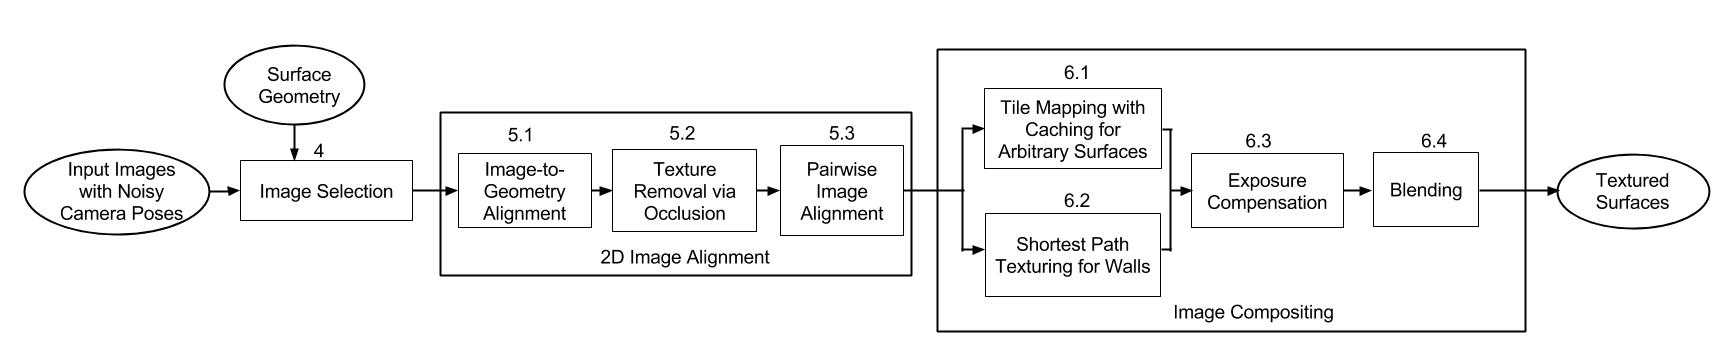
\includegraphics[width=6.2in]{flowchart2.jpg}
  \caption{The proposed texture mapping procedure\\}
  \label{fig:flowchart}
\end{figure}


The overall block diagram for the proposed texture mapping procedure
is shown in Figure \ref{fig:flowchart}, where the number attached to
each box indicates the section in which the concept in the box is
explained in this paper. First, the geometry of an environment is
split into regions, each of which will be textured independently and
in parallel. For each region, we begin by selecting a set of images
that spans the entire region's surface with high resolution
imagery. We then use recovered noisy camera poses to project these
selected images onto the surface. These projections are rotated and
translated in 2D, in order to maximally align them with the surface's
geometry, as well as to each other, allowing us to handle both errors
in geometry as well as camera poses. Finally, we demonstrate a
tile-based as well as a shortest-path-based approach for compositing
images, where the latter produces superior textures, but is only
applicable for surfaces with optimal camera poses and lateral image
coverage.

The remainder of the paper is organized as follows. Section
\ref{sec:dataAcquisition} provides background on the data acquisition
system and describes a region segmentation procedure. Section
\ref{sec:relatedWork} covers existing approaches to image stitching,
and their performance on our datasets. Section
\ref{sec:imageSelection} explains how to downsample the set of
available images by selecting those with the best orientation and
distance from surfaces under consideration. Section
\ref{sec:2dAlignment} contains the proposed approach towards 2D image
alignment, followed by Section \ref{sec:imageCompositing}, which
describes two methods of selecting and compositing images to create
the final texture. Sections \ref{sec:results} and \ref{sec:conclusion}
contain results and conclusions.

\section{Data Acquisition}
\label{sec:dataAcquisition}

This section contains background information describing the
backpack-mounted system and its operation. The hardware and operation
of the backpack system, as well as the postprocessing of acquired
data, play an important role in motivating the approaches described in
this paper. The following two sections will focus on image and raw
data acquisition, and a method of partitioning recovered environment
geometry, respectively.

\subsection{Acquisition Hardware}

The backpack system used in this paper has a number of laser range
scanners as well as side-facing cameras taking photos at a rate of 5
Hz \cite{liu2010indoor}. In order to collect data, an operator wears
the backpack system and traverses the environment to be scanned,
walking in straight lines at a standard pace and making an effort to
walk parallel to all walls in the area. Multiple localization and
loop-closure algorithms are then applied to the raw data collected by
the onboard sensors \cite{chen2010indoor, kua2012loopclosure,
  liu2010indoor}, and the backpack is localized\footnote{In this
  paper, we use the terms localization and pose recovery
  interchangeably, in that they both refer to recovering position and
  orientation.}  over its data collection period. This involves
recovering the 6 degrees of freedom for the backpack itself as well as
the cameras rigidly mounted on it. These results are noisy, which
motivates the approaches in this paper. Once this is complete, the
data from the laser range scanners is used to generate a 3D point
cloud of the surrounding environment. This point cloud is used to
construct simple, coarse models \cite{sanchez2012point,
  turnerfloorplan}, as well as highly detailed models
\cite{turnerwatertight}.  Regardless of resolution or size,
the model, consisting of geometric surfaces in 3D space, along with
the set of images captured by the backpack's cameras and their noisy
3D poses, are the input to the texture mapping problem.

\subsection{Geometry Partitioning}
\label{sec:geometryPartitioning}

\begin{figure}
  \centering
  \subfloat[][]{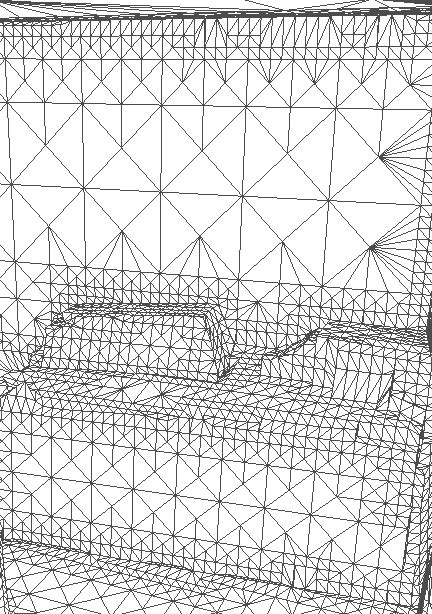
\includegraphics[width=1.5in]{geomdeskwire_crop.png}}
  \hspace{0.5in}
  \subfloat[][]{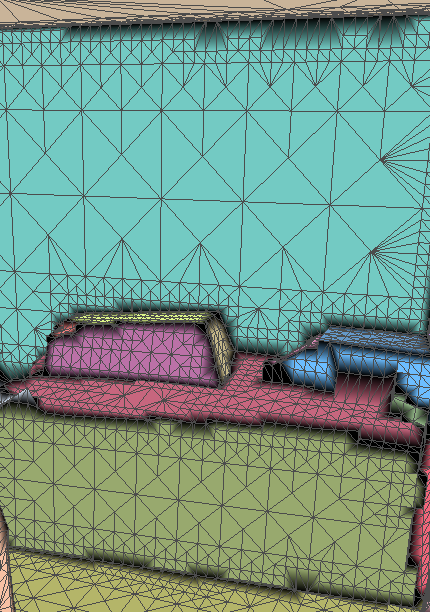
\includegraphics[width=1.5in]{geomdeskregions_crop.png}}
  \hspace{0.5in}
  \subfloat[][]{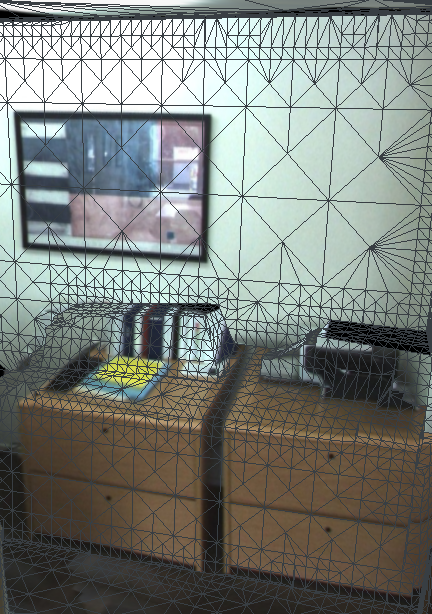
\includegraphics[width=1.5in]{geomdesktexturetris_crop.png}}
  \caption{(a) Part of a model representing a desk and miscellaneous
    objects on top of the desk. (b) Triangles grouped into regions for
    texturing. (c) Final textured output.}
  \label{fig:deskGeom}
\end{figure}


In order to effectively texture a 3D model, we first divide the model
into a set of regions, each to be textured independently. The purpose
of this is to ensure texture continuity along large uniform areas,
while allowing texture boundaries to fall along natural environmental
boundaries. Because textures may not match at such boundaries where
two regions meet, it is important to minimize the visibility of
boundaries. This is done by encouraging region boundaries to occur at
sharp corners in the model geometry, where texture continuity is not
important. For instance, in Figure \ref{fig:deskGeom}(a), each side of
the desk, objects on top of the desk, and the wall behind, should be
textured separately. This is done by grouping the triangles comprising
each such area into separate regions. Region grouping is performed by
first designating all contiguous coplanar groups of triangles as
different regions. Any regions that are less than $1 m^2$ in size are
then repeatedly joined to their largest neighboring regions, as long
as the angle between them is under $90^{\circ}$. An example of such a
grouping is shown in Figure \ref{fig:deskGeom}(b). The same area with
textures successfully applied to each region is shown in Figure
\ref{fig:deskGeom}(c).

For the purposes of texturing, it is convenient to treat each region
as planar. To accomplish this, a plane is fitted to each region. This
plane corresponds to the largest contiguous section of coplanar
triangles, as most regions are characterized by small outcroppings
from a largely planar surface, such as objects on a table or features
protruding from a wall. The 3D surface composing a region is then
projected onto its calculated plane, and the resulting 2D planar
polygon is used as the texturing surface. This 2D planar approximation
provides a simple, yet approximately accurate surface onto which
images can be projected in order to generate textures. However, 3D
surfaces are still retained in order to achieve accurate results when
performing occlusion checks, and of course are used to generate the
final textured model. Each region now has a set of triangles
representing the original model geometry, as well as a planar
approximation. The task now is to generate a texture for each region.

\section{Related Work}
\label{sec:relatedWork}

\begin{figure}
  \centering \subfloat[][]{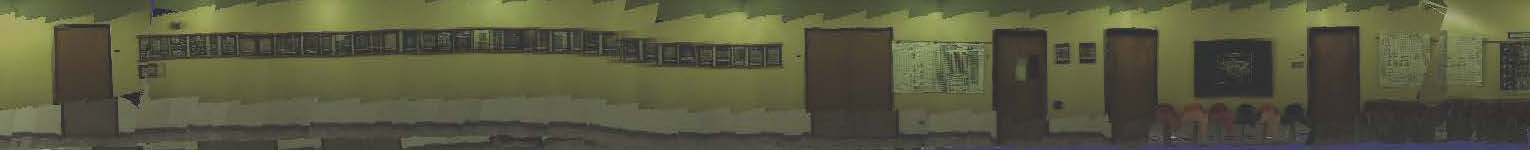
\includegraphics[trim=0cm 0cm 20cm 0cm,
    clip=true, width=6in, height=0.7in]{graphApproach.jpg}}

  \centering \subfloat[][]{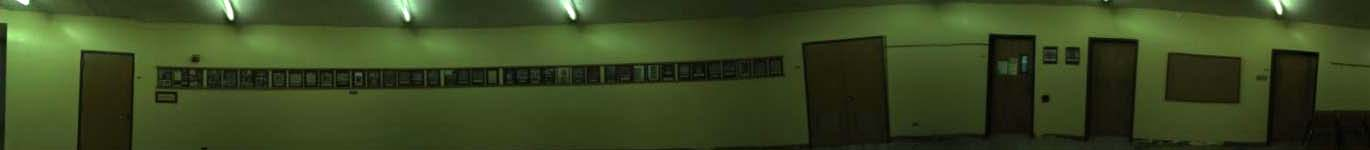
\includegraphics[trim=0cm 0cm 15cm 0cm,
    clip=true, width=6in, height=0.7in]{autostitchResult.jpg}}

  \centering \subfloat[][]{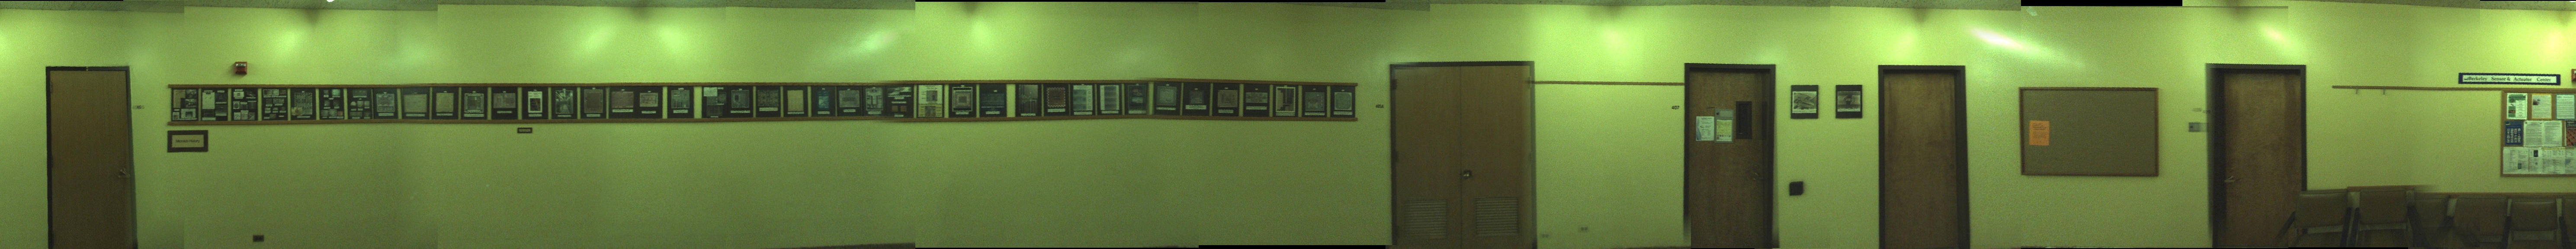
\includegraphics[trim=0cm 0cm 75cm 0cm,
    clip=true, width=6in, height=0.7in]{finalLong.jpg}}

  \caption{Texture alignment via (a) the graph-based localization
    refinement algorithm, (b) the AutoStitch software package, and (c)
    the method proposed in this paper.}
  \label{fig:mosaic3D}
\end{figure}

There are many existing approaches to stitching together multiple
images to produce a larger, seamless image \cite{szeliski2006image,
  agarwalapanoramas, wangmultipleviews, coorg1997matching,
  debevechybrid, bernardinimultiplescans}. Generally, parts of images
are matched to each other, by detecting feature points and identifying
matches. Images are then transformed to maximizally align matches,
often by computing homographies between pairs of images, or by
iteratively adjusting camera poses in 1 to 6 degrees of freedom.

Feature matching works best when unique visual references exist in the
environment that can be detected in multiple images. Unfortunately,
many indoor environments have a high prevalence of bare surfaces as
well as repeating textures, such as with windows and
doors. Additionally, our datasets often contain long 1-dimensional
chains of images, such as in Figure \ref{fig:mosaic3D}, which often
leads to error accumulation. For example, when matching a long chain
of images via homography matrices, a pixel in the $nth$ image must be
translated into the first image's coordinates by multiplying by the
$3\times3$ matrix $H_1 H_2 H_3 ... H_n$. Errors in each of these
homography matrices is propagated to all further images, resulting in
drift.

Two methods based on feature matching and homography calculation are
shown in Figure \ref{fig:mosaic3D}. Figure \ref{fig:mosaic3D}(a)
depicts an attempt at integrating image stitching with the iterative
global localization algorithm used to localize the backpack system
detailed in Section \ref{sec:dataAcquisition}
\cite{liu2010indoor}. Figure \ref{fig:mosaic3D}(b) depicts an output
image from AutoStitch, which is software based on research in the
related area of panorama generation \cite{panorama2d,
  autostitch}. Both methods were thoroughly tuned for the shown
example, but due to the factors mentioned in the previous paragraph,
they still show significant amounts of drift and distortion, as well
as loss of alignment to the environment geometry.

\section{Image Selection}
\label{sec:imageSelection}

The geometry of the texture mapping process for a region, as described
in Section \ref{sec:geometryPartitioning}, is shown in Figure
\ref{fig:projection}. Given a set of images to texture a target
surface, camera matrix $P_i$ for the $i$th image transforms a 3D point
in the world coordinate system to a 2D point or pixel in image $i$'s
coordinates. A camera matrix $P_i$ is composed of the camera's
intrinsic parameters, containing focal length and image center, as
well as extrinsic parameters which specify the rotation and
translation of the camera's position in 3D world coordinates at the
time that image $i$ was taken. These extrinsic parameters are
determined by the backpack hardware and the corresponding localization
algorithms \cite{chen2010indoor, liu2010indoor, kua2012loopclosure}
and are noisy.

Since the backpack system takes pictures at a rate of 5 Hz, thousands
of images are available for texturing each surface in the 3D
model. Our objective in designing a texture mapping process is to
determine which of these images should be used, and where their
contents should map onto the final texture, in order to minimize any
visual discontinuities or seams that would suggest that the plane's
texture is not composed of a single continuous image. In the remainder
of this section, we propose an image subsampling procedure to obtain a
set of images for use in all further steps.

\begin{figure}
  \begin{minipage}[b]{0.45\linewidth}
    \centering
    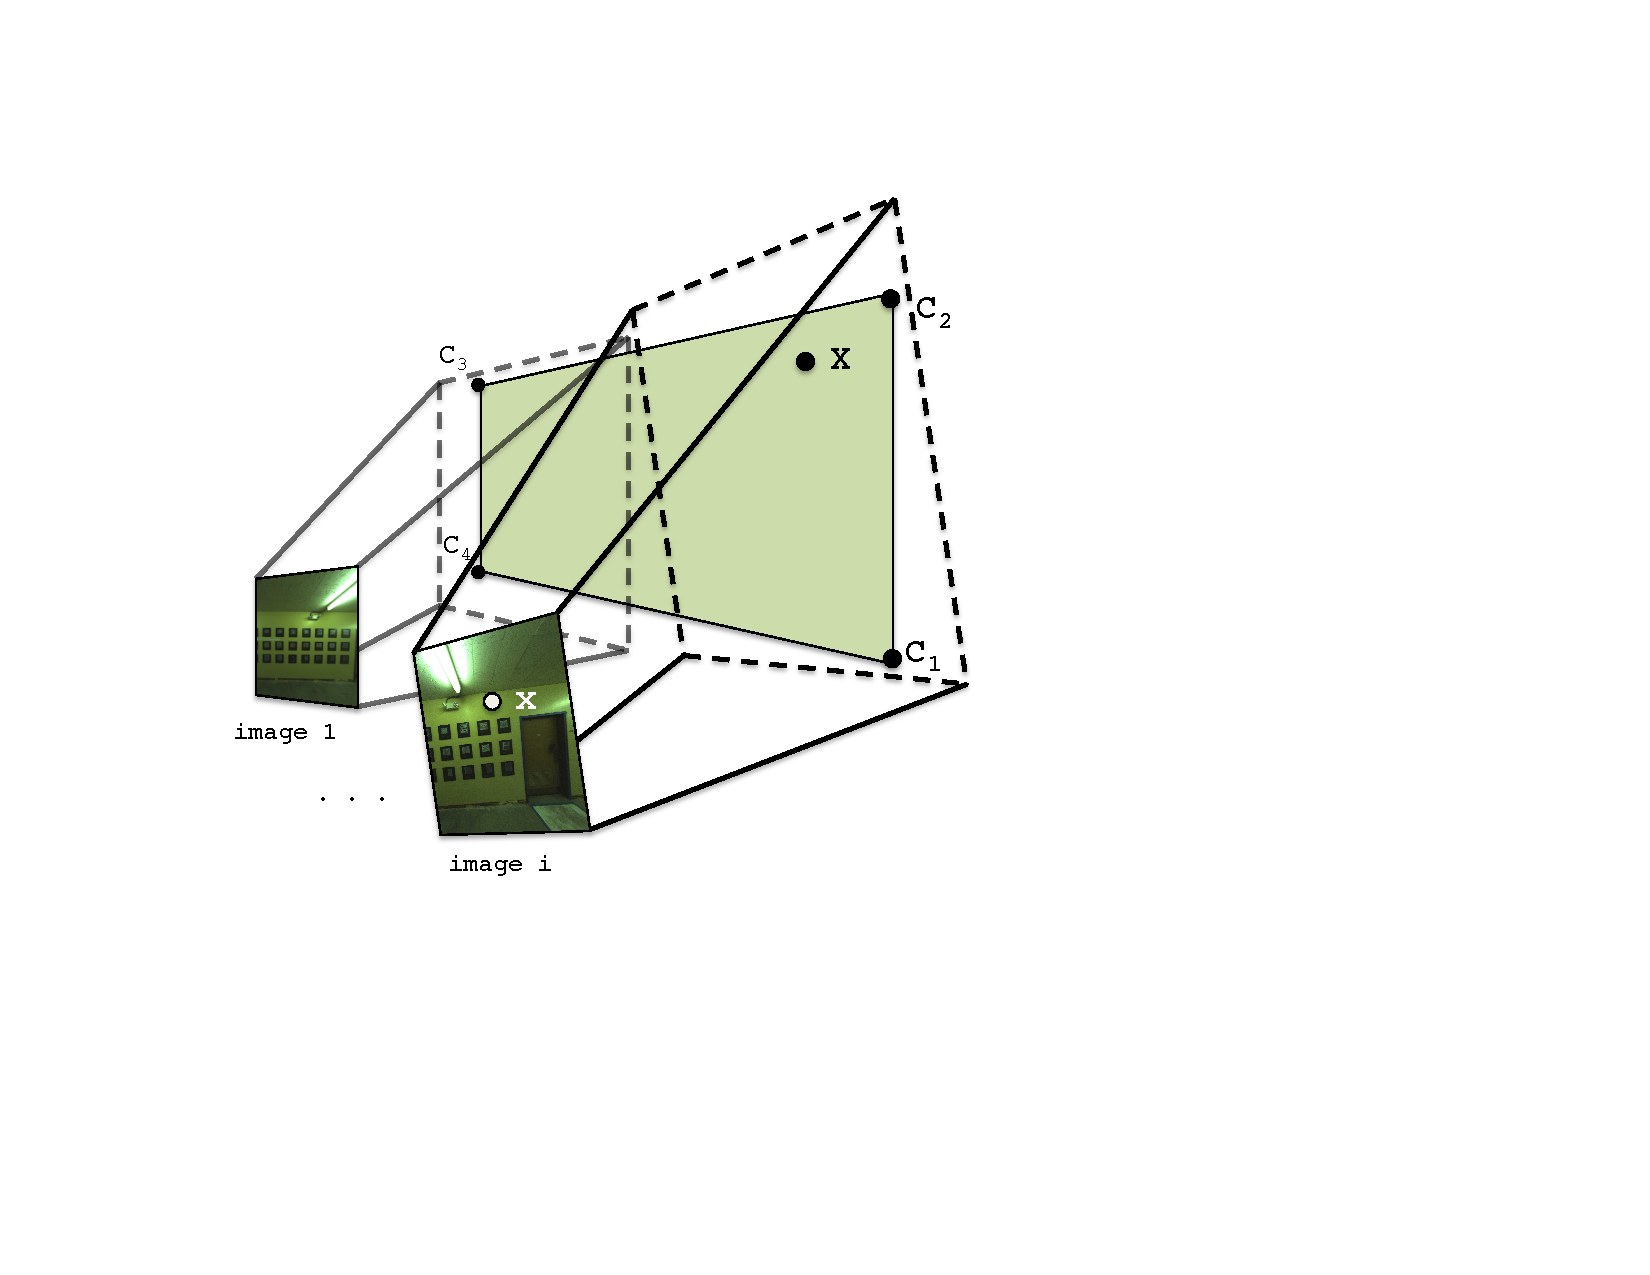
\includegraphics[height=1.5in]{Projection.pdf}
    \caption{Images are related to each surface through the camera
      matrices $P_{1..m}$. }
    \label{fig:projection}
  \end{minipage}
  \hspace{0.5cm}
  \begin{minipage}[b]{0.45\linewidth}
    \centering
    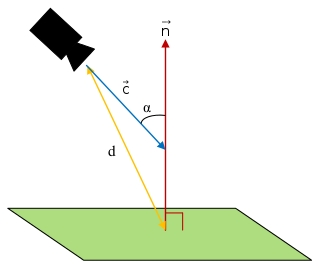
\includegraphics[height=1.5in]{scoringFunction.jpg}
    \caption{Camera angle $\alpha$ and distance $d$ are minimized by
      maximizing the scoring function $\frac{1}{d} (-1 \cdot \vec{c})
      \cdot \vec{n}$}
    \label{fig:scoringFunction}
  \end{minipage}
\end{figure}


Our criteria for image subsampling has the following
stipulations. First, we want a set of images such that their
projections together cover up the entirety of our target surface, so
as to avoid holes in the final texture. Second, we desire our final
texture to have high resolution throughout; thus every location on the
target surface should have at least one image that contains high
resolution imagery for it. A straightforward way to accomplish these
goals is to discretize the target surface into small square tiles, and
for each tile, select the image that has the best viewing angle and
resolution for texturing that tile. In order to select the image that
can best texture a tile $t$, we first gather a list of candidate
images that contain all four of its corners; we can rapidly check this
by projecting $t$ into each image using the $P_i$ camera
matrices. Furthermore, each candidate image must have been taken at a
time when its camera had a clear line-of-sight to $t$, which can be
determined using standard ray-polygon intersection tests between the
camera location, $t$, and every other surface, or via the k-d tree
from Section \ref{sec:geometryPartitioning} if present
\cite{rayintersection}.

Once we have a list of candidate images for $t$, we define a scoring
function in order to objectively select the best image for texturing
$t$. Since resolution decreases and camera pose errors become more
pronounced with distance, we wish to minimize the distance between
cameras and the surfaces they texture. Additionally, we desire images
that are projected perpendicularly, rather than obliquely, onto the
plane, maximizing the resolution and amount of useful texture
available in their projections, as well as minimizing any parallax
effects due to real-world geometry not accurately represented by the
digital 3D model. In other words, we wish to minimize the angle
between the tile's normal vector and the camera axis for images
selected for texturing that tile. These two criteria can be met by
maximizing the function $\frac{1}{d} (-1 \cdot \vec{c}) \cdot \vec{n}$
as shown in Figure \ref{fig:scoringFunction}, where $d$ is the
distance between the centers of a camera and a tile, and $\vec{n}$ and
$\vec{c}$ are the directions of the plane's normal and the camera axis
respectively.

When the images selected for each tile are used directly to texture
their respective tiles, image boundaries with abrupt discontinuities
between tiles are visible, as shown in Figure
\ref{fig:compareAll}(a). While it is clear that camera pose
inaccuracies are too severe for such a simple approach to work, the
selected images all appear to contain optimal camera angles with high
resolution, and much of their misalignment appears reconcilable using
2D transforms. This procedure generally selects around 10\% of the
possible images that could be used for texturing a surface, and not
only reduces the computational complexity of the remaining steps, but
also selects the most promising images for the remaining steps.



\begin{figure}
  \centering \subfloat[][]{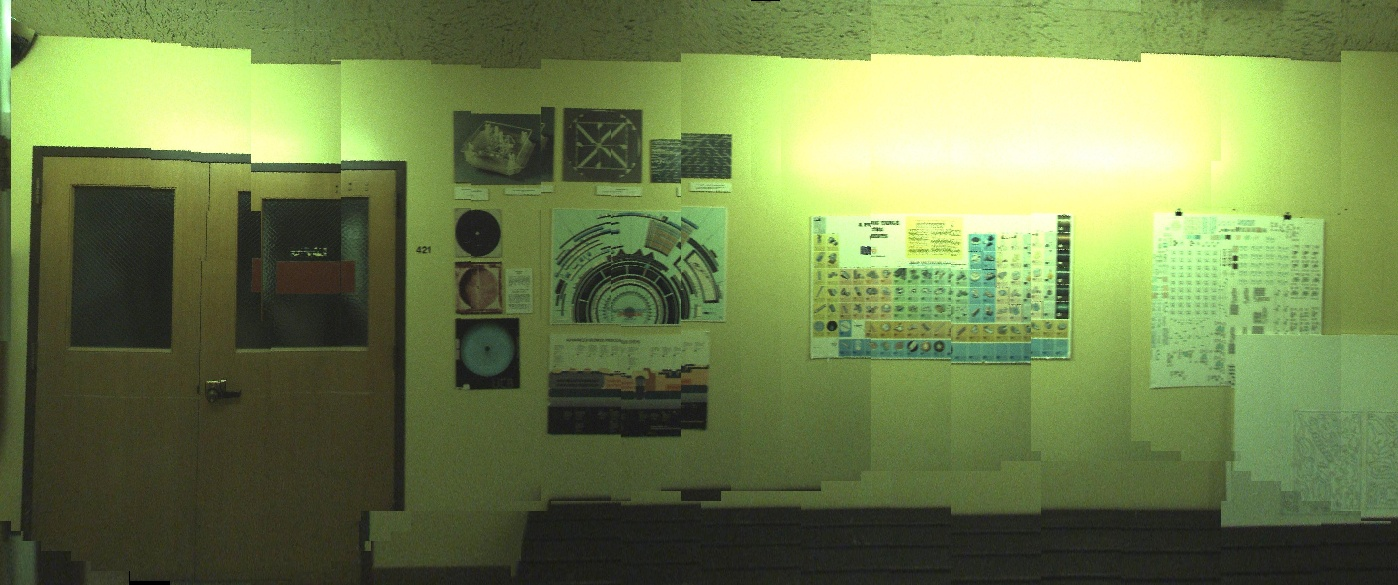
\includegraphics[width=0.33\textwidth,
    height=0.8in]{wall2_naive.jpg}}
  \subfloat[][]{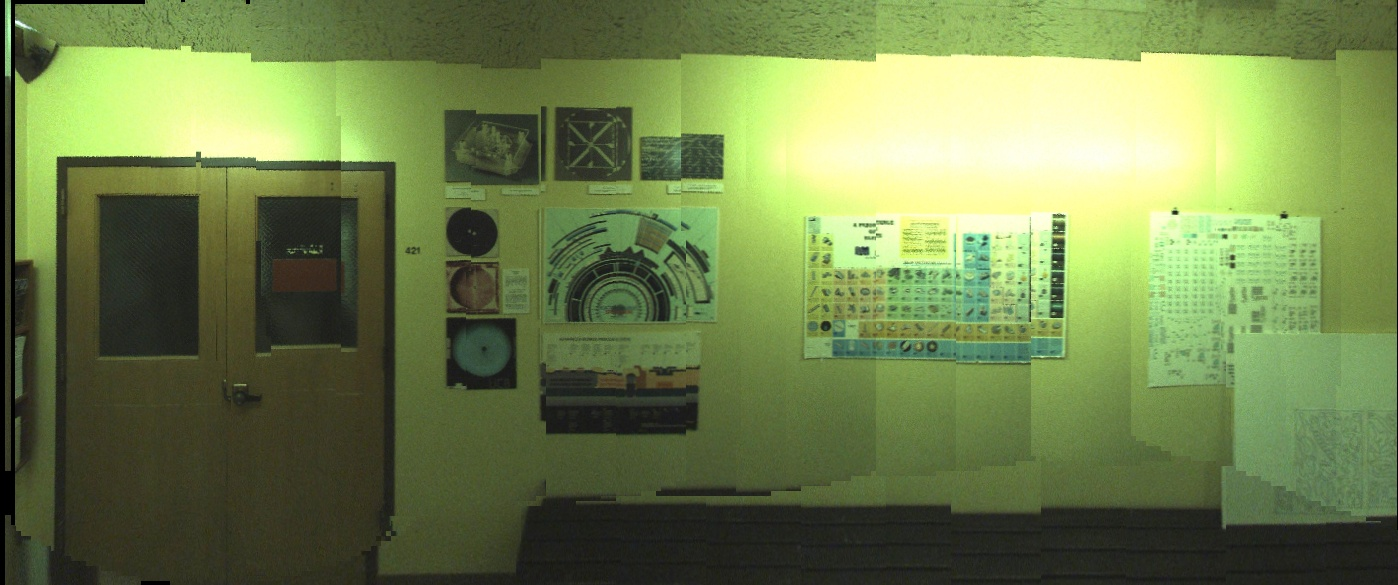
\includegraphics[width=0.33\textwidth,
    height=0.8in]{wall2_naive_shift.jpg}}
  \subfloat[][]{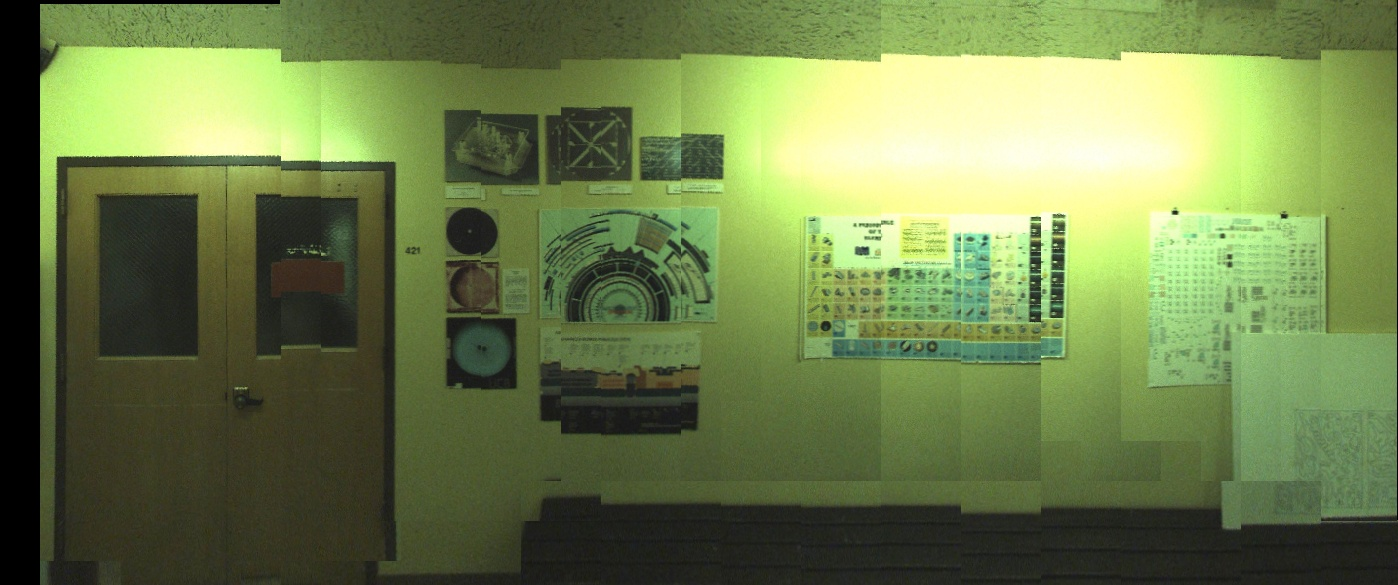
\includegraphics[trim=1.2cm 0cm 0cm 0cm,
        clip=true,width=0.33\textwidth,
    height=0.8in]{wall2_cache_shift.jpg}}

  \centering \subfloat[][]{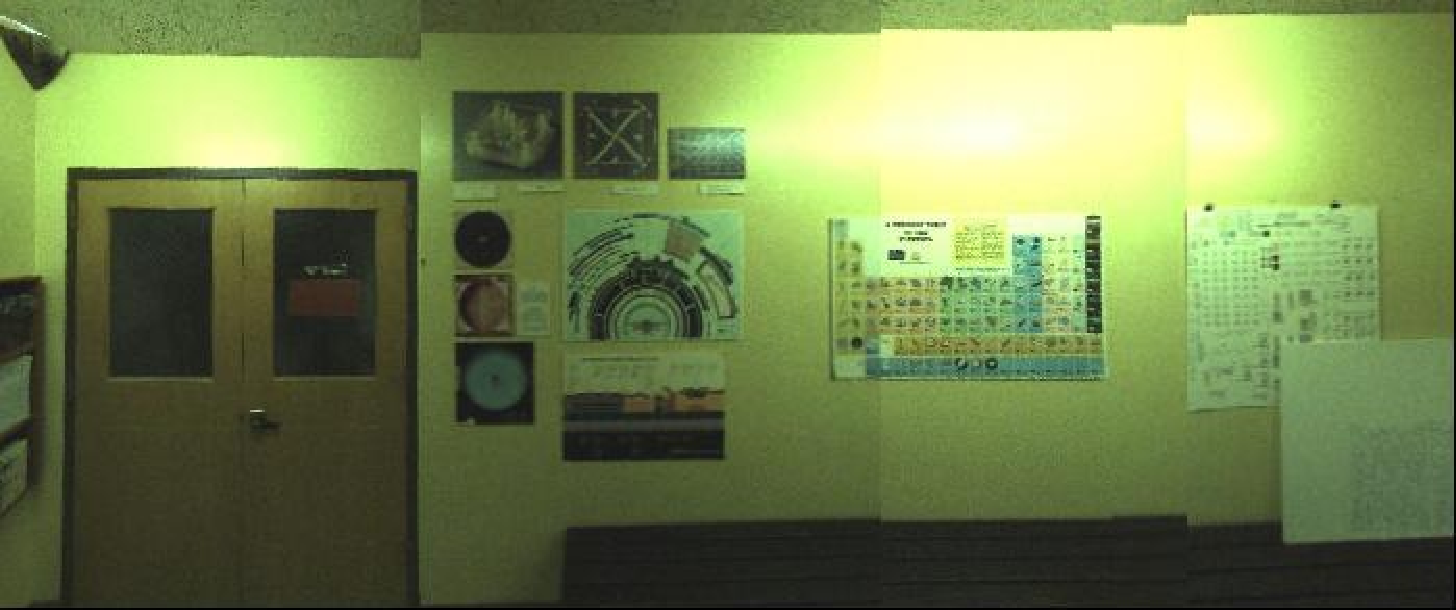
\includegraphics[width=0.33\textwidth,
    height=0.8in]{wall2_shortest_shift.pdf}}
  \subfloat[][]{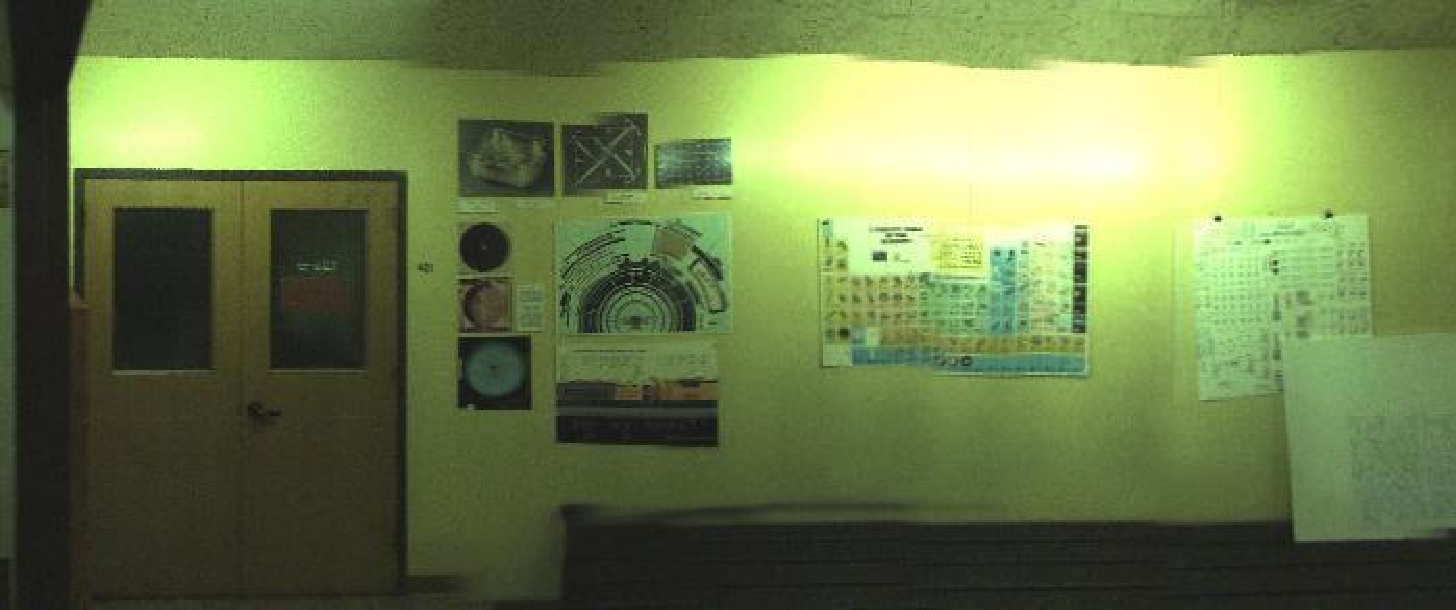
\includegraphics[width=0.33\textwidth,
    height=0.8in]{wall2_cache_shift_blend.pdf}}
  \subfloat[][]{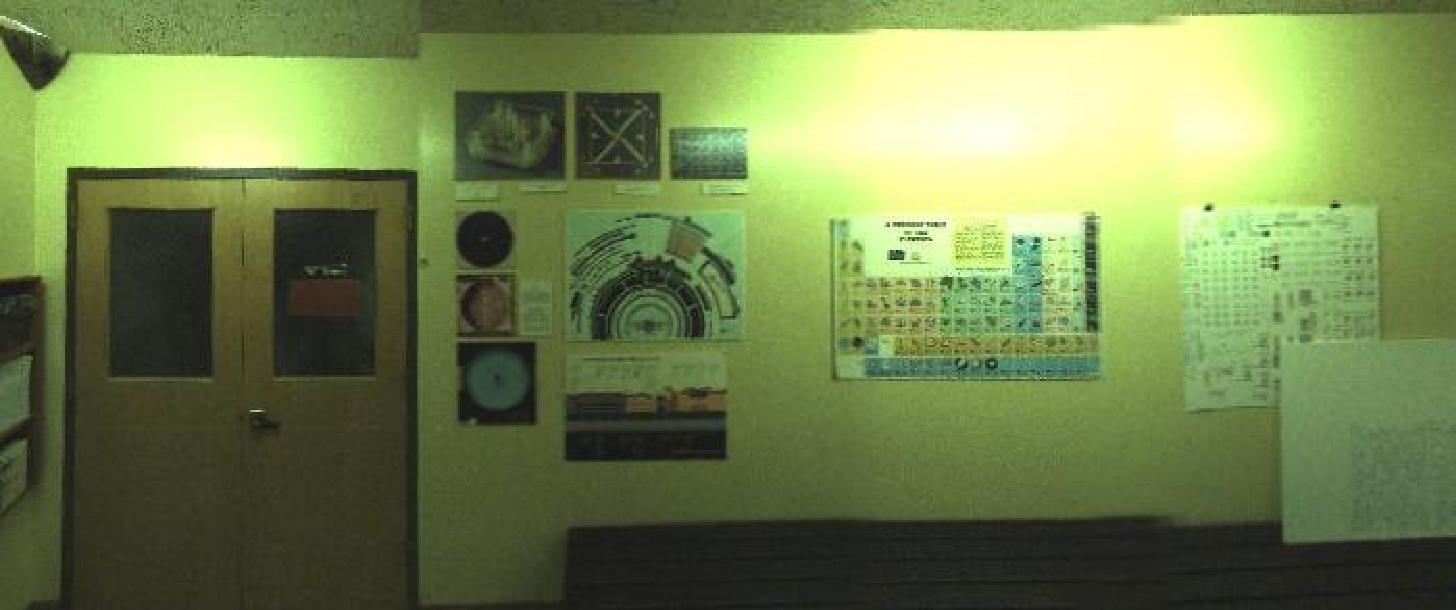
\includegraphics[width=0.33\textwidth,
    height=0.8in]{wall2_shortest_shift_blend.pdf}}

  \caption{(a) Tile-based texturing; (b) Tile-based texturing after
    image alignment; (c) Tile-based texturing after image alignment
    with caching; (d) Shortest path texturing after image alignment;
    (e,f) Blending applied to (c) and (d).}
  \label{fig:compareAll}
\end{figure}


\section{2D Image Alignment}
\label{sec:2dAlignment}
In this section, we describe our method for efficient and robust image
alignment. Rather than register all of our images in 3D, as many
state-of-the-art techniques for image stitching do, we instead align a
subset of images in 2D; this subset corresponds to the images selected
by the image selection procedure described in Section
\ref{sec:imageSelection}.

Applying 2D alignments to this set of images works well for the
following reasons. First, the nature of our input data and the
selected images is such that localization error chiefly occurs in two
dimensions, which correspond to the plane of most surfaces being
projected onto. This is because the backpack operator, while scanning
an environment, generally walks parallel to walls. Furthermore, the
backpack system maintains a consistent distance from floors and
ceilings during data collection. As a result, the translational error
of camera poses is quite minimal in dimensions perpendicular to walls,
ceilings and floors, which comprise the majority of surfaces being
textured.

Our proposed 2D alignment procedure consists of three parts, as shown
in the diagram in Figure \ref{fig:flowchart}. First, images are
projected onto the surface and lines within these projected images are
detected. Images are then transformed such that these lines match
geometric lines composing the boundaries of the surface being
textured. Second, occlusion checks are performed to remove invalid
parts of each image for the target surface. Third, SIFT feature
matches are detected between pairs of images, and a weighted linear
least squares problem is solved in order to maximize all image and
geometry-based alignments.


\subsection{Geometry-based Alignment}
\label{sec:geometryAlignment}

\begin{figure}
  \centering
  \begin{tabular}{cc}
    \begin{tabular}{c}
      \subfloat[][]{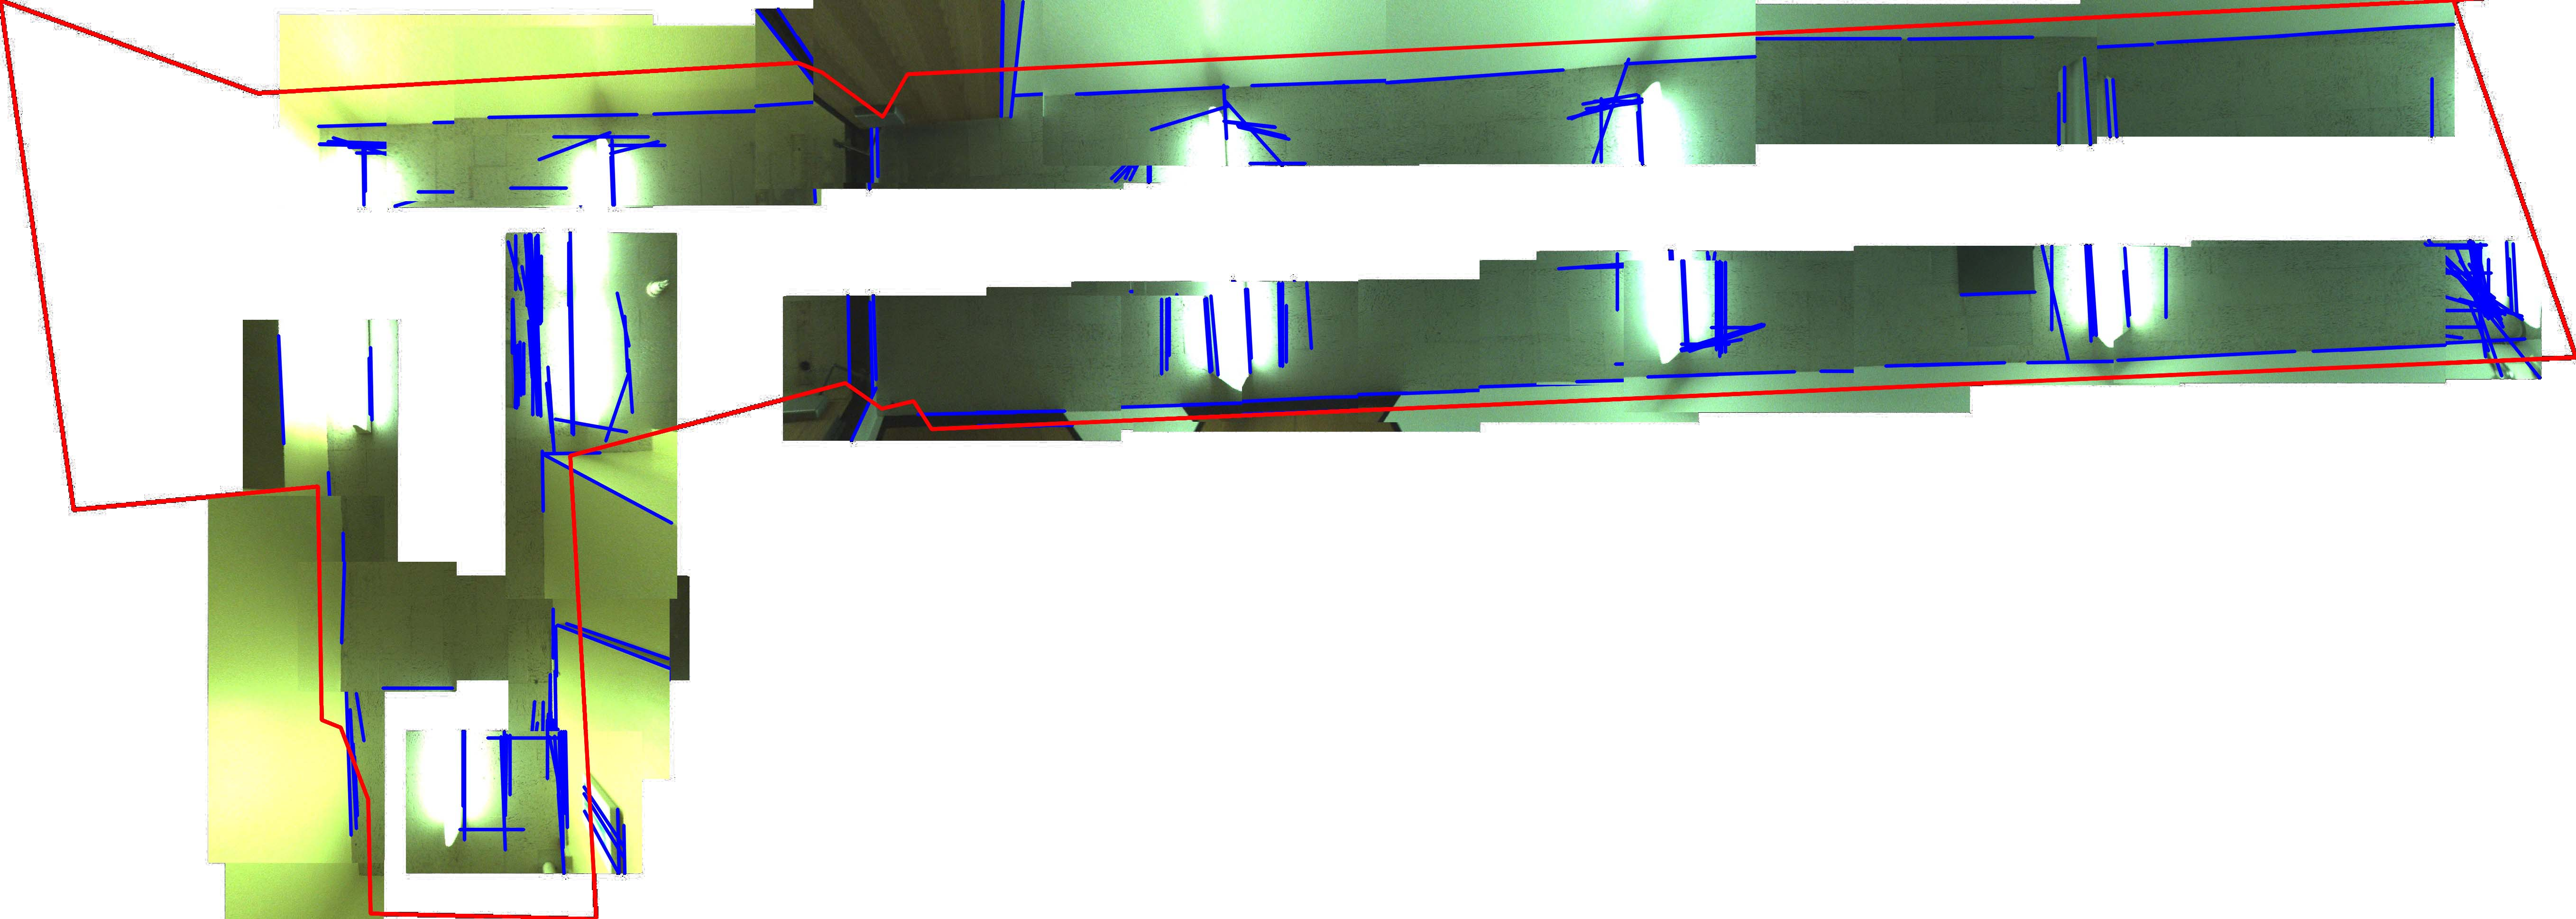
\includegraphics[trim=0cm 0cm 1.3cm 0cm,
        clip=true, width=3in,
        height=0.9in]{allunshifted.jpg}} \\
      \subfloat[][]{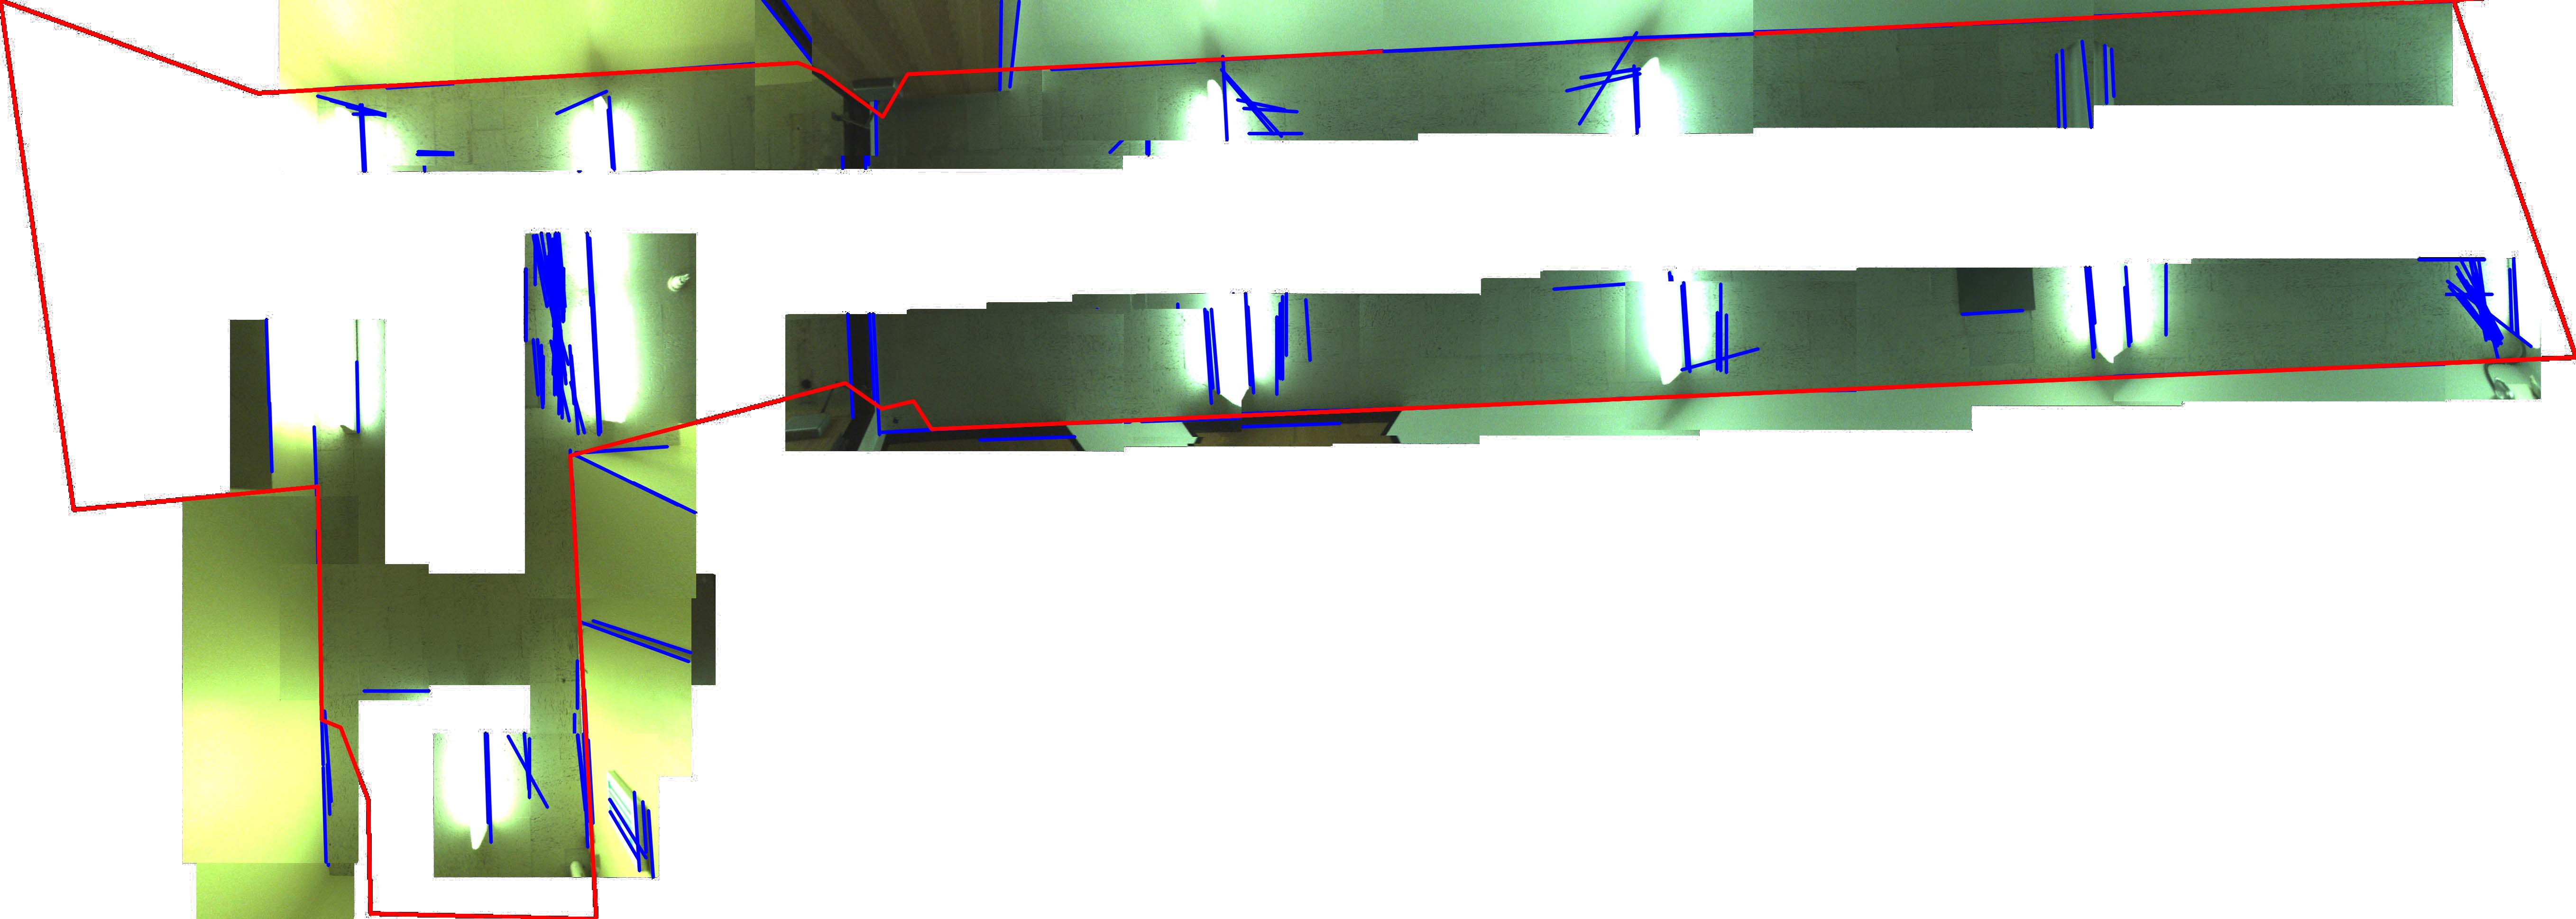
\includegraphics[trim=1.3cm 0cm 0cm 0cm,
        clip=true, width=3in,
        height=0.9in]{allshifted.jpg}}
    \end{tabular} &
    \subfloat[][]{\raisebox{-1in}{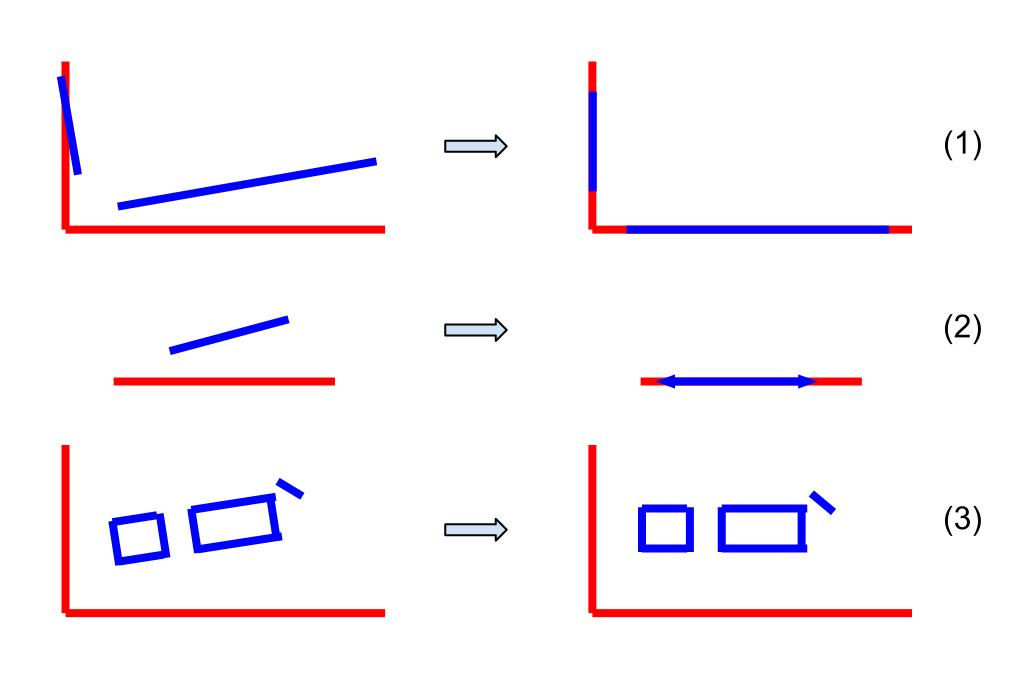
\includegraphics[width=3in]{matchLines.jpg}}} 
  \end{tabular}
  \caption{Images projected onto a ceiling surface, where
    geometry-based lines corresponding to the ceiling's boundary are
    shown in red. Image-based lines detected by Hough transform in the
    image projections are shown in blue; (a) images projected with
    their original noisy camera poses; (b) after image alignment to
    maximize line matches between images and geometry; (c) examples of
    matching lines in cases with $\geq$ 2 line pairs, 1 line pair, and
    zero line pairs, from top to bottom.}
  \label{fig:geometryAlignment}
\end{figure}


After computing each image's projection onto the target surface, as
described in Section \ref{sec:imageSelection}, we can obtain a set of
image-based line segments by using Hough transforms to detect lines in
the image projections. We also gather a set of geometry-based lines,
which correspond to the lines comprising the target surface's border,
as well as lines formed where other surfaces intersect the target
surface. An example of these lines is shown in red for a ceiling
surface in Figure \ref{fig:geometryAlignment}(a). Given perfect camera
poses and surface geometry, the lines in images corresponding to
corners between surfaces should match up exactly with corners in the
3D model. By inducing such lines to match, we can fit camera poses
more accurately to the surface, and therefore to each other as well.

To align images to surface geometry, we collect pairs of image-based
and geometry-based line segments, which are within distance and
angular thresholds of each other. We have found a distance threshold
of 250 mm and an angular difference threshold of $10^\circ$ to work
well for our datasets. For each pair of lines, we compute the angular
difference between the pair's image and geometry lines. If there are 2
or more pairs with angular differences within $1^\circ$, we select the
two pairs with the longest noncollinear image-based lines, and rotate
the image such that the lines in the pair with the longest image-based
line become parallel. We then find a translation such that the lines
in that same pair overlap. This translation has ambiguity in the
dimension along the matched lines, which is resolved by matching the
midpoint of the image-based line in the second pair to its
corresponding geometry-based line. This is shown in case (1) of Figure
\ref{fig:geometryAlignment}(c). Thus, with 2 or more pairs, it is
possible to obtain a fixed rotation and translation for geometry
alignment, which are saved for usage in Section
\ref{sec:robustSIFTFeatureMatching}.

If there are not 2 or more pairs with similar angular differences, we
select the pair with the longest image-based line, which corresponds
to a strong linear visual feature, and apply a rotation and the
minimal translation to match the pair's lines. This translation's
ambiguity however, can not be resolved, but is also saved to be used
in Section \ref{sec:robustSIFTFeatureMatching}. This is shown in case
(2) of Figure \ref{fig:geometryAlignment}(c). Finally, in the case
where there are no line pairs, we can still rotate images in order to
exploit patterns in indoor environments, as shown in case (3) of
Figure \ref{fig:geometryAlignment}(c). For instance, doors, windows,
furniture, ceiling lights, etc. tend to have linear edges that are
parallel to the edges of the surfaces they are on. Thus, we choose to
minimize the angle between image-based lines and geometry-based lines
regardless of distance. We use the RANSAC framework to compute a
rotation angle that best accomplishes this while ignoring
outliers. \cite{fischler1981random}.

After these steps, image projections line up well with target
surfaces, as shown in Figure \ref{fig:geometryAlignment}(b), which is
considerably more aligned than Figure
\ref{fig:geometryAlignment}(a). This procedure reconciles both errors
in camera poses as well as in geometry, and results in sharp,
continuous borders across images, which is crucial when checking for
occlusion.


\subsection{Image Occlusion}
\label{sec:imageOcclusion}

\begin{figure}
  \centering
  \begin{tabular}{cc}
    \subfloat[][]{\raisebox{-1in}{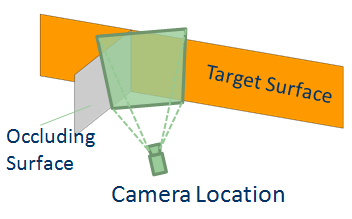
\includegraphics[width=3in]{occlusiondiagram.png}}} &
 
  \begin{tabular}{c}
    \subfloat[][]{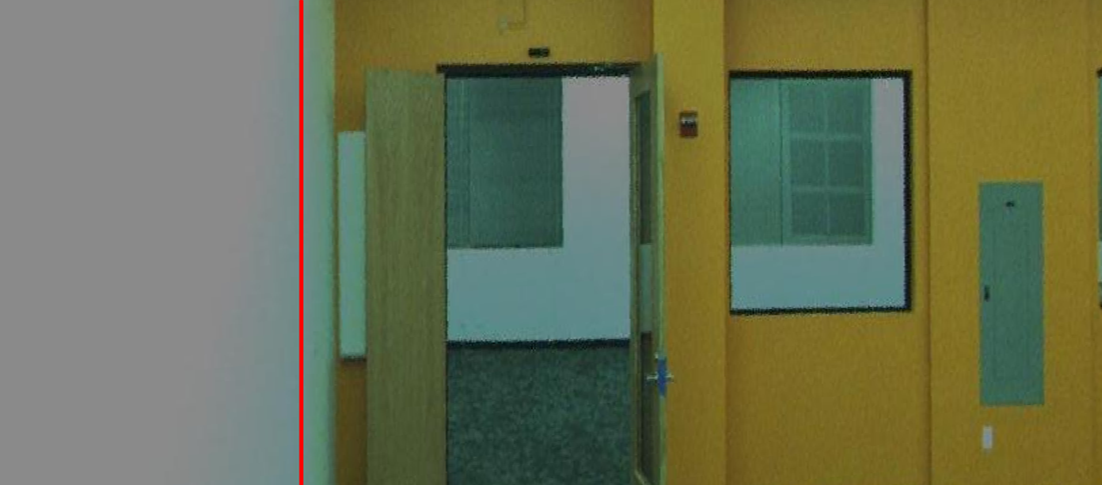
\includegraphics[trim=0cm 0cm 1.3cm 0cm,
      clip=true, width=3in,
      height=0.9in]{occlusionimagebad.png}} \\
    \subfloat[][]{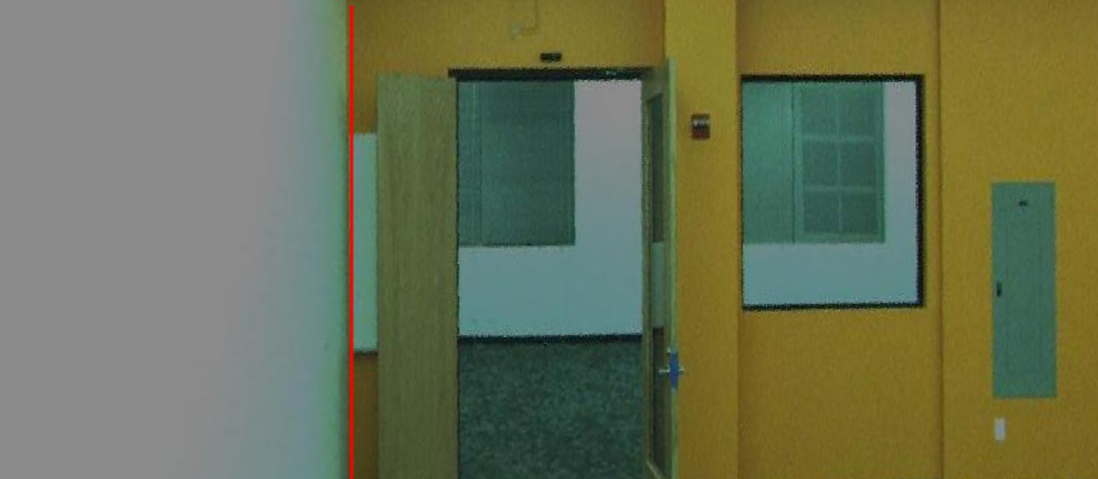
\includegraphics[trim=1.3cm 0cm 0cm 0cm,
      clip=true, width=3in,
      height=0.9in]{occlusionimagegood.png}}
  \end{tabular}
\end{tabular}
\caption{(a) The image from the camera in this diagram contains
  texture that belongs to the gray occluding surface, which should not
  be projected onto the orange target surface; (b) without geometry
  alignment, texture to the left of the red line would be removed,
  which would leave some erroneous texture projected onto our target
  surface; (c) after geometry alignment, the image is shifted,
  resulting in the correct amount of texture being removed.}
\label{fig:occlusion}
\end{figure}

In order to correctly texture surfaces, it is important to detect and
remove parts of image projections containing texture for occluding
surfaces. For instance, in Figure \ref{fig:occlusion}(a), an image
used to texture the orange target surface also contains part of a gray
occluding surface. We remove this incorrect texture by performing
ray-polygon intersection tests between the camera location and every
surface in our model except the target surface
\cite{rayintersection}. If using planar approximations for regions, as
explained in Section \ref{sec:geometryPartitioning}, the k-d tree is
used instead. These intersection tests are performed repeatedly in a
recursive grid, until all occlusions are detected and corresponding
occluded texture is removed. Occlusion checking works entirely with
geometry, so by ensuring that images match geometry using
\ref{sec:geometryAlignment}'s alignment procedure, texture belonging
to other surfaces is accurately removed, as seen in Figure
\ref{fig:occlusion}(b) vs. \ref{fig:occlusion}(c).

\subsection{2D Feature Alignment}
\label{sec:robustSIFTFeatureMatching}
The next step is to align the selected images from Section
\ref{sec:imageSelection} for each surface to each other by searching
for corresponding feature points between all pairs of overlapping
images. We use feature alignment rather than pixel or intensity-based
alignment due to the differences in lighting as well as possible
occlusion among images, both of which feature alignment is less
sensitive to \cite{lowe1999object, mikolajczyk2005performance,
  szeliski2006image}. We use SiftGPU \cite{siftgpu} for its high
performance on both feature detection as well as pairwise
matching. These matches determine $dx$ and $dy$ distances between each
pair of features for two image projections, though these distances may
not always be the same for different features. Since indoor
environments often contain repetitive features such as floor tiles or
doors, we need to ensure that SIFT-based distances are
reliable. First, we only align parts of images that overlap given the
original noisy poses. Second, we discard feature matches that
correspond to an image distance greater than 200 mm from what the
noisy poses estimate. RANSAC \cite{fischler1981random} is then used to
obtain a consensus from the the remaining feature matches.

We now use the feature-based distances between each pair of images as
well as geometry alignment results from Section
\ref{sec:geometryAlignment} to refine all image positions using a
weighted linear least squares approach. An example setup for such a problem $\textrm{min}_{\vec{\beta}}
||W^\frac{1}{2}(A \vec{\beta} - \vec{\gamma})||_2^2 $ with 3 images is
as follows.

\[
A =
\begin{pmatrix}
  -1 & 1 & 0 & 0 & 0 & 0\\
  0 & 0 & 0 & -1 & 1 & 0\\
  0 & -1 & 1 & 0 & 0 & 0\\
  0 & 0 & 0 & 0 & -1 & 1\\
  0 & -m_2 & 0 & 0 & 1 & 0\\
  1 & 0 & 0 & 0 & 0 & 0\\
  0 & 0 & 0 & 1 & 0 & 0\\
  1 & 0 & 0 & 0 & 0 & 0\\
  0 & 0 & 0 & 1 & 0 & 0\\
  0 & 1 & 0 & 0 & 0 & 0\\
  0 & 0 & 0 & 0 & 1 & 0\\
  0 & 0 & 1 & 0 & 0 & 0\\
  0 & 0 & 0 & 0 & 0 & 1\\


\end{pmatrix}\quad
\vec{\beta} =
\begin{pmatrix}
  x_1, \\ x_2, \\ x_3, \\ y_1, \\ y_2, \\ y_3
\end{pmatrix}
\vec{\gamma} =
\begin{pmatrix}
  dx_{1,2}, \\ dy_{1,2}, \\ dx_{2,3}, \\ dy_{2,3}, \\ -m_2gx_2 + gy_2,
  \\ gx_1, \\ gy_1, \\ tx_1, \\ ty_1, \\ tx_2, \\ ty_2, \\ tx_3, \\
  ty_3
  
\end{pmatrix}
\vec{W} =
\begin{pmatrix}
  1, \\ 1, \\ 1, \\ 1, \\ 1, \\ 1, \\ 1, \\ 0.01, \\ 0.01, \\ 0.01, \\
  0.01, \\ 0.01, \\ 0.01
\end{pmatrix}
\]


The variables to solve for are the $x_i$ and $y_i$ positions
of images, while equations are the feature-based distances between
pairs of images, images fixed to geometry with 0 or 1 degrees of
freedom, and the original noisy camera poses. In this scenario, a
feature-based distance of $dx_{1,2}$, $dy_{1,2}$ was calculated
between images 1 and 2. This corresponds to the first and second row
of $A$, while the third and fourth row of $A$ represent the same for
images 2 and 3. Rows 5 through 7 correspond to results of the geometry
alignment procedure in Section
\ref{sec:geometryAlignment}. Specifically, row 5 corresponds to a
geometry-based constraint of image 2's location to a line of slope
$m_2$, passing through point $gx_2$, $gy_2$, while rows 6 and 7
correspond to a fixed location for image 1 without any degrees of
freedom. Rows 8 through 13 correspond to the original camera locations
for each image ($tx_i,ty_i$).

The original camera poses are needed due to lack of feature matches in
all images, or lack of enough geometry alignment results to generate a
single solution. Since it is desirable to minimally use the original
noisy poses, we assign to them a weighting factor of $0.01$, while all
other equations are weighted at $1$.

Since this problem is linear, it can be solved efficiently; after
applying the resulting shifts, images overlap and match each other
with far greater accuracy. Using the simple tile-based texturing
scheme from Section \ref{sec:imageSelection} on these adjusted images
results in Figure \ref{fig:compareAll}(b), which has far fewer
discontinuities than in \ref{fig:compareAll}(a), though some 3D error
as well as lighting differences and parallax effects are still
visible.

\section{Image Compositing}
\label{sec:imageCompositing}
In Section \ref{sec:imageSelection} we described an image selection
method, that when used to create a texture, resulted in many visible
discontinuities. In Section \ref{sec:mappingWithCaching}, we will
refine that approach with an added caching mechanism to improve
texture continuity. This method works well for all arbitrary camera
poses and surfaces. However, for cases where images have consistently
perpendicular viewing angles to surfaces under consideration, such as
walls, we develop an alternative method in Section
\ref{sec:shortestPath} which further reduces visual artifacts. Both of
these approaches are then combined with an exposure compensation and
blending scheme in order to produce final textures for each surface.

\subsection{Tile-Mapping with Caching}
\label{sec:mappingWithCaching}
For the simple texturing method described in Section
\ref{sec:imageSelection}, discontinuities occur where adjacent tiles
are textured by different images. Though Section
\ref{sec:2dAlignment}'s image alignment removes many such
discontinuities, there are still cases where seams are visible due to
imprecise matching or other factors such as model-based errors. To
reduce this, we implement a spatiotemporal caching mechanism to take
into account image selections made by neighboring tiles while texture
mapping a given tile. By using the same image across tile boundaries,
it is possible to eliminate a discontinuity altogether. If a tile is
not visible in images used by neighboring tiles, using similar images
across tile boundaries still leads to less noticeable discontinuities.

The best image for a tile $t$ is selected by searching through two
subsets of images for a viable candidate, before searching through the
entire set of valid images obtained in Section
\ref{sec:imageSelection}. The first subset of images is those selected
by adjacent tiles that have already been textured. We must first check
which of these images contain texture for $t$, and then of those, we
make a choice according to the scoring function in Figure
\ref{fig:scoringFunction}. Before reusing this image, we check the
criteria $\alpha < 45^\circ$, in order to ensure a high resolution
projection, with $\alpha$ as the camera angle as shown in Figure
\ref{fig:scoringFunction}.

If no satisfactory image is found in the first subset, we check a
second subset of images, consisting of those taken near the ones in
the first subset, both spatially and temporally. We use the noisy
camera poses to determine spatial proximity. These images are not the
same as the ones used for neighboring tiles, but are taken at a
similar location and time, suggesting that their localization and
projection are quite similar, and thus likely match more
seamlessly. If no viable image is found according to the $\alpha <
45^\circ$ criteria, we search the entire set of candidate images from
Section \ref{sec:imageSelection}, selecting based on the same scoring
function from Figure \ref{fig:scoringFunction}.

The result of applying this caching approach to the images for the
surface in Figure \ref{fig:compareAll}(a) is shown in Figure
\ref{fig:compareAll}(c), where seams are considerably reduced as
compared to Figure \ref{fig:compareAll}(b). However, some
discontinuities are still present, as visible in the posters on the
wall with breaks in their borders.


\subsection{Shortest Path Texturing}
\label{sec:shortestPath}

\begin{figure}
  \centering
  \begin{minipage}{3in}
    \centering
    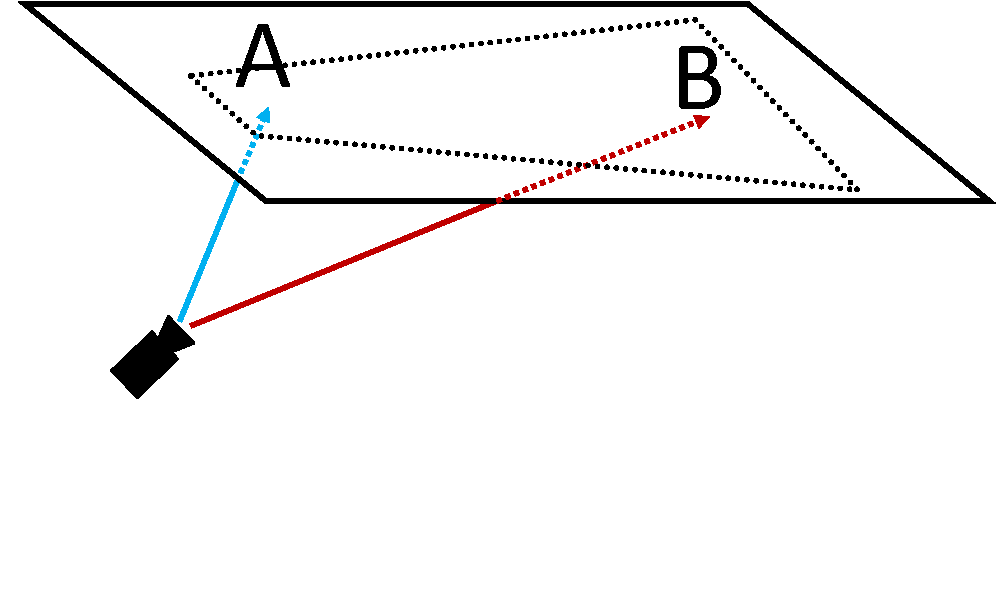
\includegraphics[width=1.5in]{projectionCeiling.pdf}
    \captionof{figure}{Camera axes for horizontal surfaces are at
      large angles with respect to plane normals.}
    \label{fig:projectionCeiling}
  \end{minipage}%
  \hspace{0.5in}
  \begin{minipage}{3in}
    \centering
    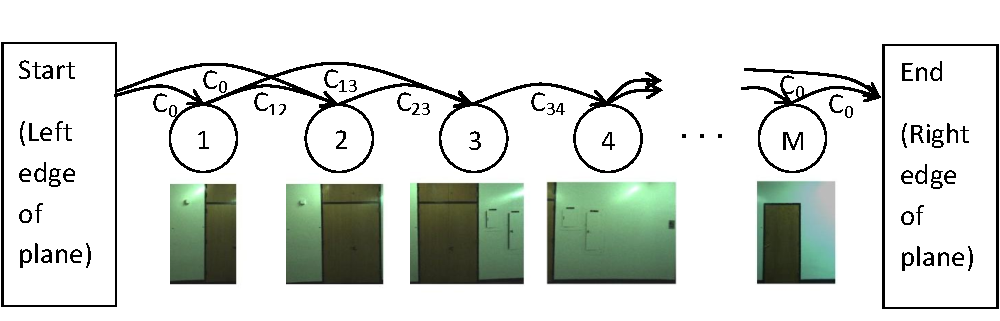
\includegraphics[width=3in]{dagCreation.pdf}
    \captionof{figure}{DAG construction for the image selection
      process.}
    \label{fig:dagCreation}
  \end{minipage}
\end{figure}

As mentioned earlier, our data comes from a mobile backpack system
with side-facing cameras. While these cameras have a wide-angle field
of view,they are often pointed directly at vertical surfaces during
data acquisition. This means that image projections on vertical
surfaces tend to have higher, and more consistent resolution, while
the more oblique projections onto horizontal surfaces result in
textures spanning large areas, such as in Figure
\ref{fig:projectionCeiling}. Using the tile-based texture mapping
criteria from Figure \ref{fig:scoringFunction}, such projections have
highly varying scores depending on the location of a tile on the
plane. Thus, the tiling approach in Section
\ref{sec:mappingWithCaching} is an appropriate choice for texturing
horizontal surfaces, as it uses the parts of image projections that
maximize resolution for their respective plane locations, e.g. areas
near point A and not near point B, in Figure
\ref{fig:projectionCeiling}.

For vertical surfaces however, which make up a large portion of most
models, images are usually taken from close distances and head-on
angles, resulting in high resolution rectangular projections. As a
result, for each tile on a wall plane, the scoring function of Figure
\ref{fig:scoringFunction} is relatively flat with respect to candidate
images, as they are all more or less head on. Since the scoring
function is less discriminative for walls, we devise a different
texturing strategy to directly minimize visible seams when texturing
them. This is done by choosing a subset of images such that their
projections (a) cover the entire plane and (b) have minimal
differences in overlapping regions. A straightforward cost function
that accomplishes the latter is the sum of squared differences (SSD)
of pixels in overlapping regions between all pairs of
images. Minimizing this cost function encourages image boundaries to
occur either in featureless areas, such as bare walls, or in areas
where images match extremely well.

To find the subset of images that covers the plane with minimal cost,
we form a shortest path problem. This can be done because the
wide-angle cameras have full floor-to-ceiling coverage of walls, and
the backpack operator logically only moves horizontally. We thus are
only concerned with lateral coverage when working with wall
surfaces. We can therefore construct a horizontal Directed Acyclic
Graph (DAG) from the images, with edge costs defined by the SSD cost
function, and solve a simple shortest path problem to find an optimal
subset of images with regard to the SSD cost function \cite{dijkstra}.


Figure \ref{fig:dagCreation} demonstrates the construction of a DAG
from overlapping images of a hallway wall. Images are sorted by
horizontal location left to right, and become nodes in a
graph. Directed edges are placed in the graph from left to right
between overlapping images. The weights of these edges are determined
by the SSD cost function. Next, we add two artificial nodes, one start
node representing the left border of the plane, and one end node
representing the right border of the plane. The left(right) artificial
node has directed edges with equal and arbitrary cost $C_0$ to(from)
all images that meet the left(right) border of the plane. We now solve
the shortest path problem from the start node to the end node. This
results in a set of images completely covering the plane horizontally,
while minimizing the cost of seams between images.

We have now (a) mapped every location on the plane to at least one
image, (b) decreased the number of texturing images, generally
retaining around 20\% of the image subset obtained in Section
\ref{sec:imageSelection}, and (c) decreased the discontinuities at
each image border. As seen in Figure \ref{fig:compareAll}(d), this
shortest path method has fewer visible discontinuities than Figure
\ref{fig:compareAll}(c) corresponding to the tile caching
approach\footnote{In Figure \ref{fig:compareAll}(d), we arbitrarily
  chose one image for texturing where images overlap, as blending will
  be discussed in section \ref{sec:blending}.}. This is especially
evident when comparing the posters in the images. This shortest path
approach approach directly reduces the cost of each image boundary,
while the tile caching method uses a scoring function that only
approximates this effect. Furthermore, this approach guarantees the
best selection of images to minimize seams, while the sequential tile
caching method may select images early on that turn out to be poor
choices once subsequent tiles have been processed. This shortest path
approach is also far less intensive in terms of memory usage and
runtime, both during texture generation and rendering, as it does not
require discretizing planes or images.

When texturing our models, we apply the shortest path method on
surfaces where images are taken at optimal angles and provide full
coverage along one dimension. Floors, ceilings, and smaller complex
objects such as furniture, given their many images taken at oblique
angles, are textured using the tile caching method of Section
\ref{sec:mappingWithCaching}.

\subsection{Exposure Compensation}
\label{sec:exposureCompensation}

\begin{figure}
  \centering
  \subfloat[][]{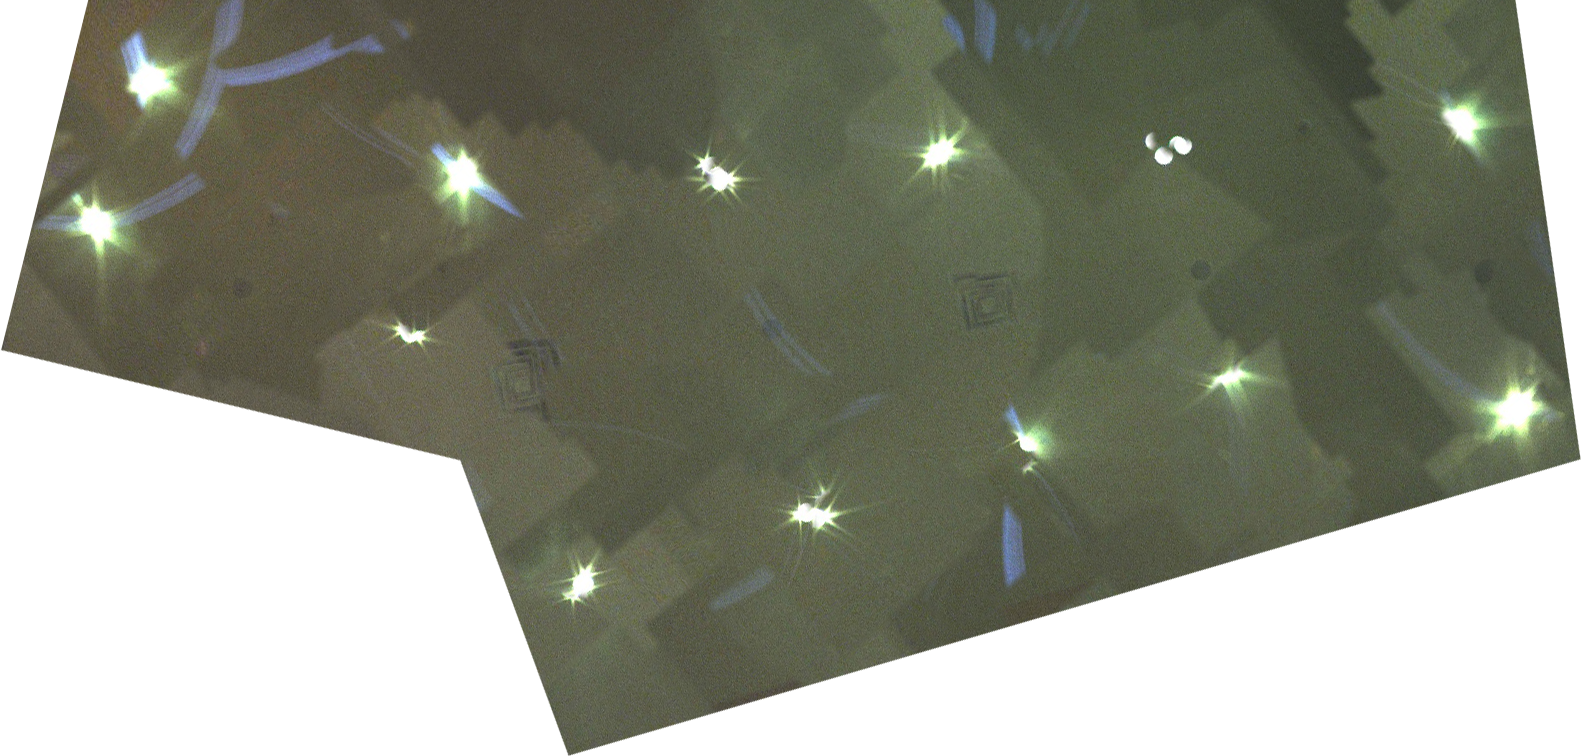
\includegraphics[width=2.5in, height=0.9in]{exposureDiff1.png}}
  \hspace{0.5in}
  \subfloat[][]{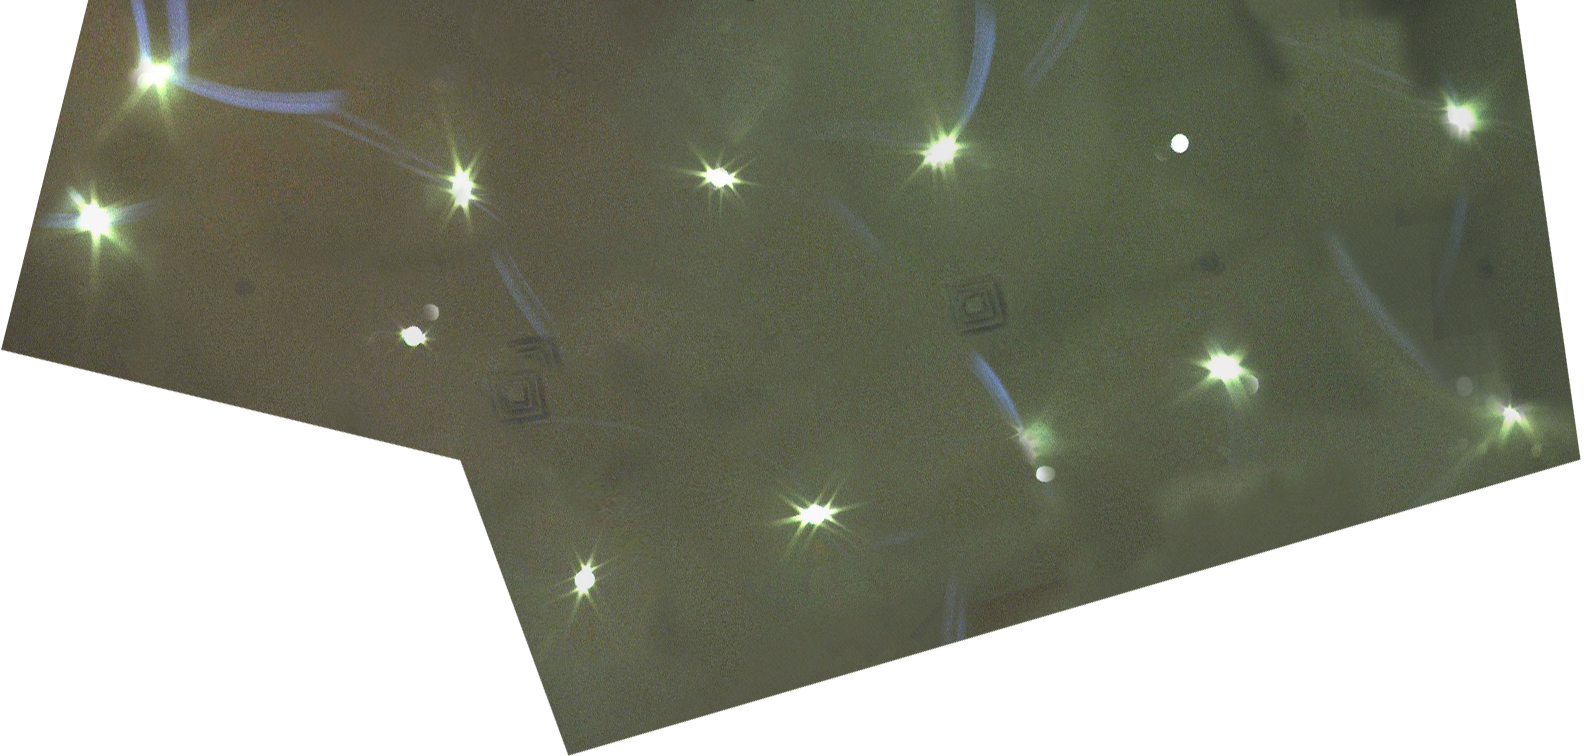
\includegraphics[width=2.5in, height=0.9in]{exposureDiff2.png}}
  \caption{(a) A ceiling texture composed of images taken with varying
    exposures, with significant brightness differences. (b) Exposure
    compensation applied to the same set of images from (a) by
    applying computed gains to each image}
  \label{fig:exposureDiff}
\end{figure}


Before blending images together, exposure compensation is applied to
equalize brightness among neighboring images. For the images in this
report, cameras are set to have automatic exposure, which means that
images of the same object may have different brightness levels. While
successful image alignment and blending can reduce sharp seams between
adjacent images, there may still be noticeable brightness gradients
between images, particularly in areas near light sources. This can be
seen in Figure \ref{fig:exposureDiff}(a), where the ceiling texture
has patches of clearly differing brightness. To diminish this effect,
a gain can be computed and applied to each image, with the effect of
linearly scaling the brightness of each image. The goal is to compute
a gain for each image, such that the brightness of an area is
consistent across image boundaries.

Similar to the image position refinement procedure in Section
\ref{sec:robustSIFTFeatureMatching}, exposure compensation is
performed simulatenously across all images present in a single
region. To begin, a relative gain $R_{ij}$ is computed for each pair
of overlapping images $I_i$ and $I_j$, which have a set of pixels
common to both images, labeled as $P_{ij}$. The relative gain $R_{ij}$
is then obtained by calculating the scaling factor between the average
intensity of $P_{ij}$ in $I_i$ and the average intensity of $P_{ij}$
in $I_j$.

As before, these pair-wise observations can be combined and solved as
a least-squares optimization problem. In this case, observations do
not need to be weighted, and so the formulation is
$\textrm{min}_{\vec{b}} ||(X \vec{b} - \vec{a})||_2^2 $. An example
setup for 3 images, where each image overlaps with both of the other
images, is shown below.
\[
X =
\begin{pmatrix}
  R_{12} & -1 & 0\\
  R_{13} & 0 & -1\\
  0 & R_{23} & -1\\
  1 & 1 & 1\\

\end{pmatrix}\quad
\vec{b} =
\begin{pmatrix}
  G_1, \\ G_2, \\ G_3
\end{pmatrix}
\vec{a} =
\begin{pmatrix}
  0, \\ 0, \\ 0, \\ 3
\end{pmatrix}
\]

In this problem, $\vec{b}$ is the $N\times1$ vector of gains $G_i$ to
be solved for, where $N$ is the number of images.  Matrix $X$ is an
observation matrix corresponding to the relative intensities of
overlapping images. In particular, the number of rows of $X$ is one
plus the number of unique pairs of overlapping images, and the number
of columns of $X$ is equal to $N$. Each row of $X$, except the last
one, contains an $R_{ij}$ value which is placed in column $i$, as well
as a $-1$ value in column $j$, with zeroes elsewhere. As explained
above, $R_{ij}$ is the relative gain between images $i$ and $j$, and
therefore $G_iR_{ij} - G_j = 0$.  Thus, all values of $\vec{a}$, which
is a vector with size equal to the number of rows of $X$, are set to
$0$, except for the last one.

The last row of $X$ and corresponding last entry of $\vec{a}$ are used
to constrain the problem, as without them, all computed gains would be
allowed to scale by any amount. To keep gains at reasonable values,
the final observation is used: $\Sigma G_i = N$, where $N$ is the
number of images. This has the effect of setting the average of all
gains to 1, and is represented by the final row of ones in $X$, and
the corresponding $N$ value in $\vec{a}$.

For the 81 source images that compose the ceiling location in Figure
\ref{fig:exposureDiff}, the corresponding $X$ matrix has 1343 rows,
and the optimization problem takes under a second to solve, on a 2.8
GHz dual core machine.  The result of computing and applying gains can
be seen in Figure \ref{fig:exposureDiff}(b). As compared to Figure
\ref{fig:exposureDiff}(a), the effect is clear, as dark/bright patches
are no longer present, and the overall brightness of the image has not
changed significantly.

\subsection{Blending}
\label{sec:blending}
We now apply a blending procedure to the texturing methods in Sections
\ref{sec:mappingWithCaching} and \ref{sec:shortestPath}. Although the
image alignment and selection steps in both methods attempt to
minimize all mismatches between images, and exposure compensation
minimizes brightness differences, there are occasional unavoidable
discontinuities in the final texture due to parallax effects or
inaccuracies in model geometry. These can however be treated and
smoothed over by applying alpha blending over image seams.  Whether
the units to be blended are rectangularly-cropped images or
rectangular tiles, we can apply the same blending procedure, as long
as there is a guaranteed overlap between units to blend over.

For the tile caching method of Section \ref{sec:mappingWithCaching},
we can ensure overlap by texturing a larger tile than needed for
display. For example, for a rendered tile of size $l_1 \times l_1$, we
can associate it with a texture $(l_1 + l_2) \times (l_1 + l_2)$ in
size.  We have found $l_2 = \frac{l_1}{2}$ to provide a good balance
between blending and keeping features unblurred at image
boundaries. For the shortest path method, we already have ensured
overlap between images. To enforce consistent blending however, we add
a minimum required overlap of images of 200 mm while solving the
shortest path problem in Section \ref{sec:shortestPath}. Additionally,
if images overlap in a region greater than the overlap distance, we
only apply blending over an area equal to the overlap distance.

After linear alpha blending across overlapping regions, the texture
mapping process is complete. Figures \ref{fig:compareAll}(e) and
\ref{fig:compareAll}(f) show the blended versions of Figures
\ref{fig:compareAll}(c) and \ref{fig:compareAll}(d) respectively. By
comparing all images, it is clear that Figure \ref{fig:compareAll}(f)
has the best visual quality and the best texturing approach among the
textures in Figure \ref{fig:compareAll}.



\section{Results}
\label{sec:results}
This section contains results of the proposed texture mapping process
on a number of different environments, with geometry generated using
three different methods. Further images of individual textured
surfaces and entire textured models, as well as videos and interactive
walkthroughs can also be found at
\footnote{\url{http://www-video.eecs.berkeley.edu/research/indoor/}}.

\subsection{Examples}
\label{sec:examples}

\begin{figure}
  \centering{
    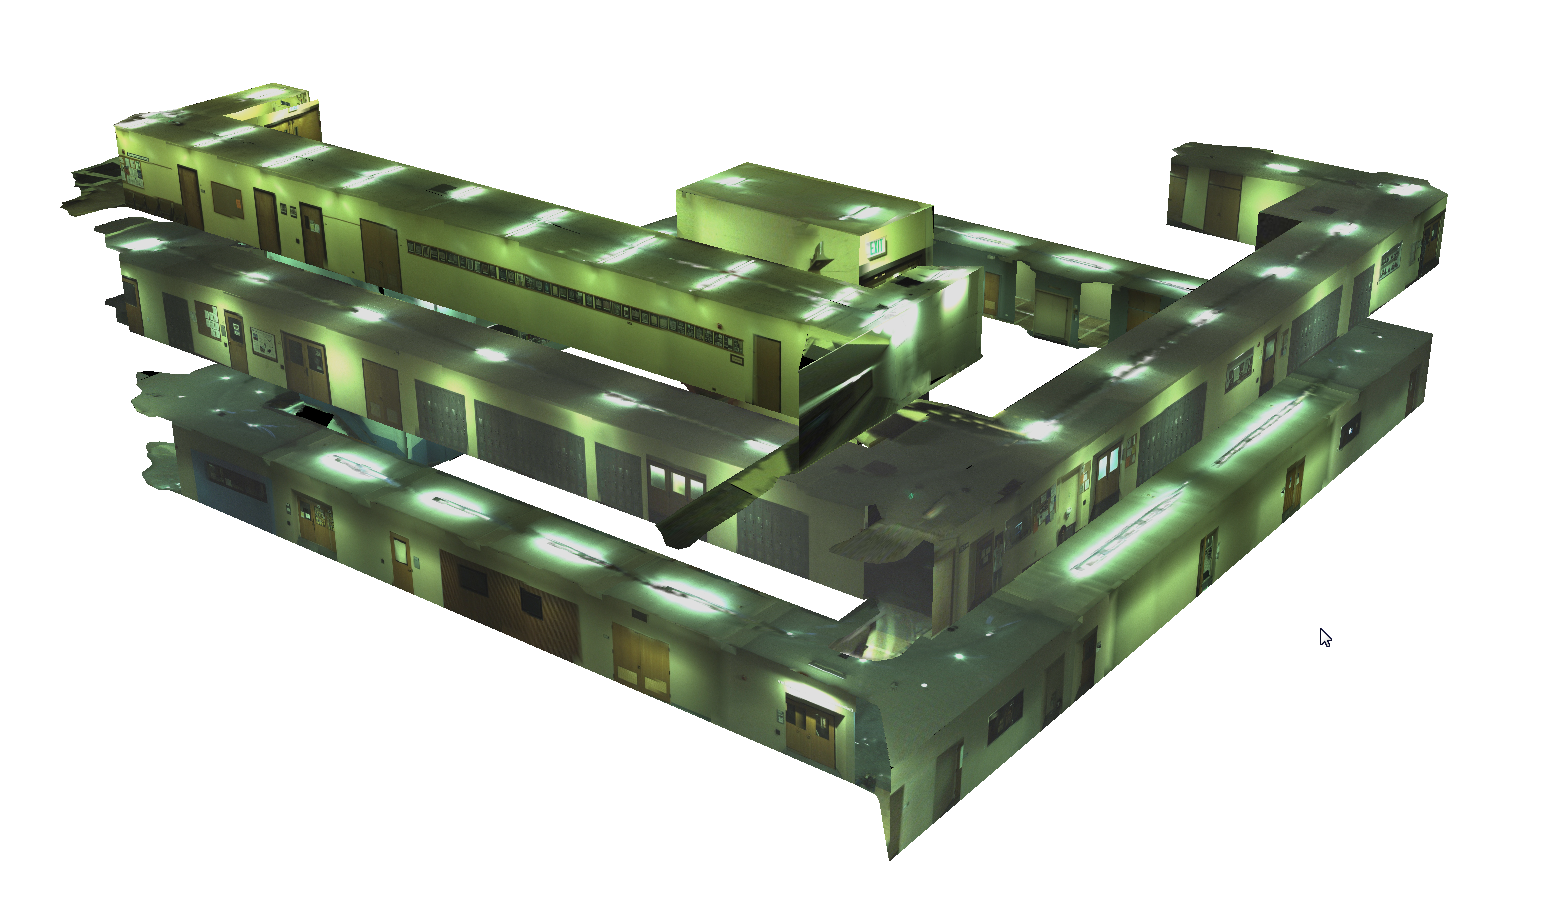
\includegraphics[width=3in]{threestoryfull2.png}
    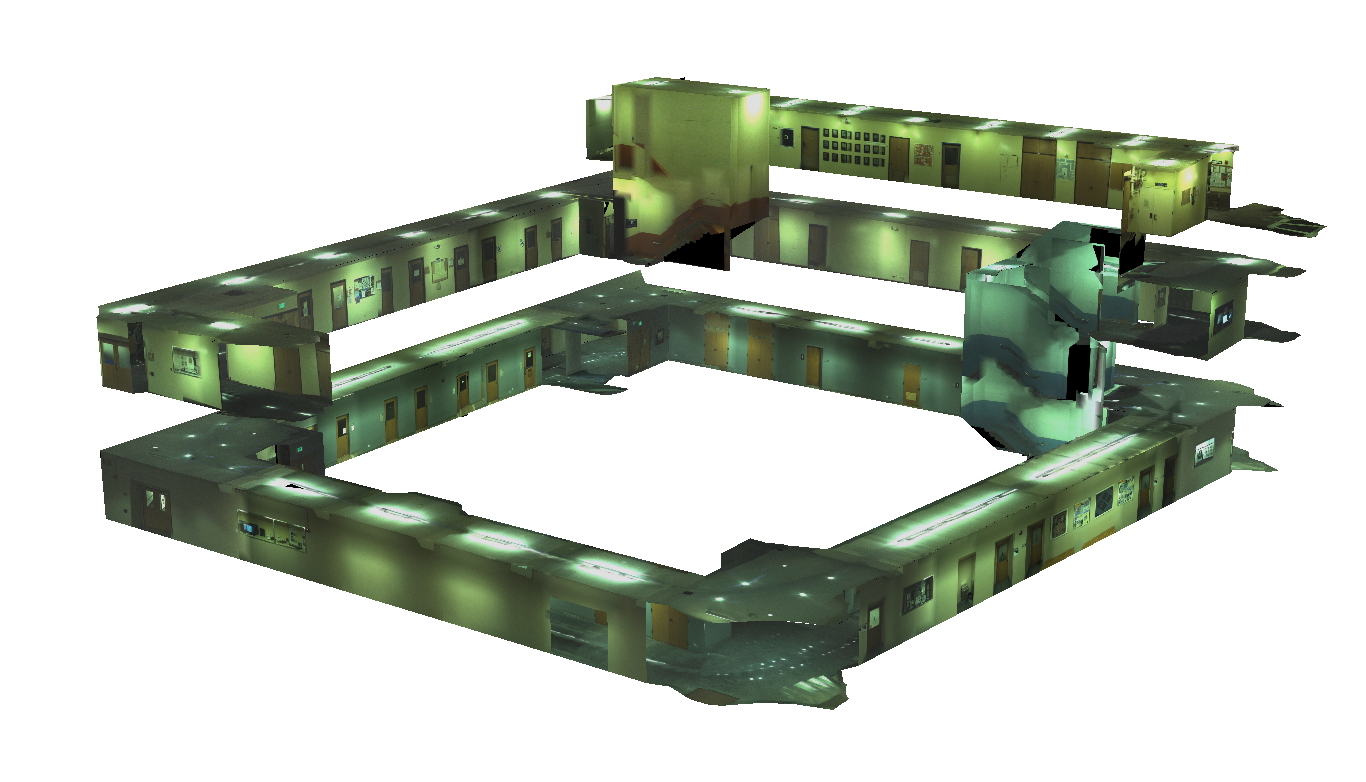
\includegraphics[width=3in]{threestoryfull.png} \\
    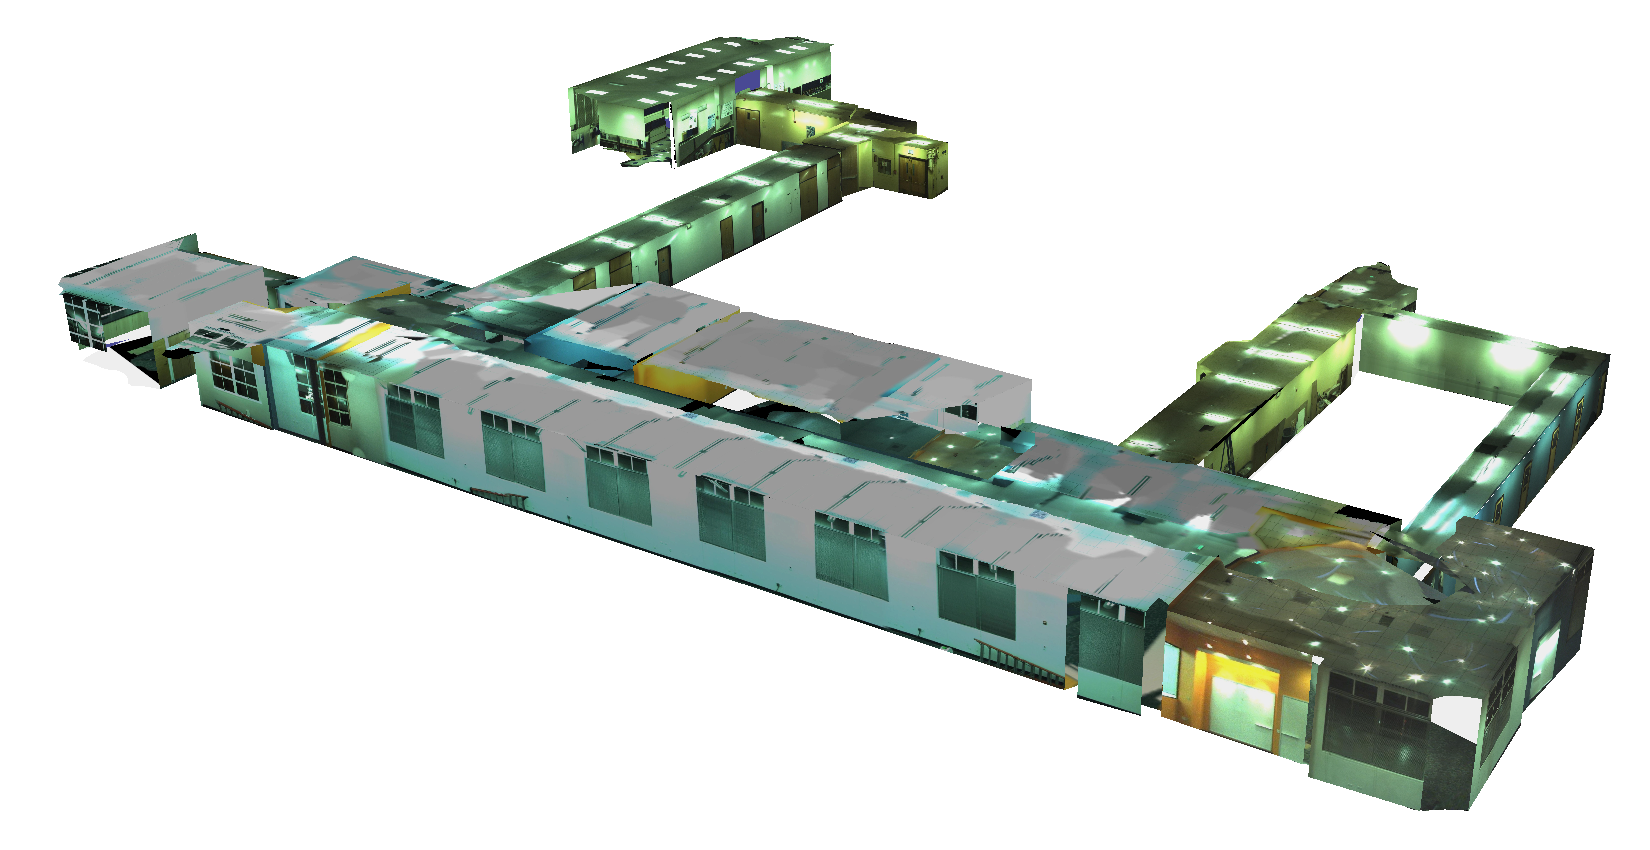
\includegraphics[width=3in]{fullmodel.png}
    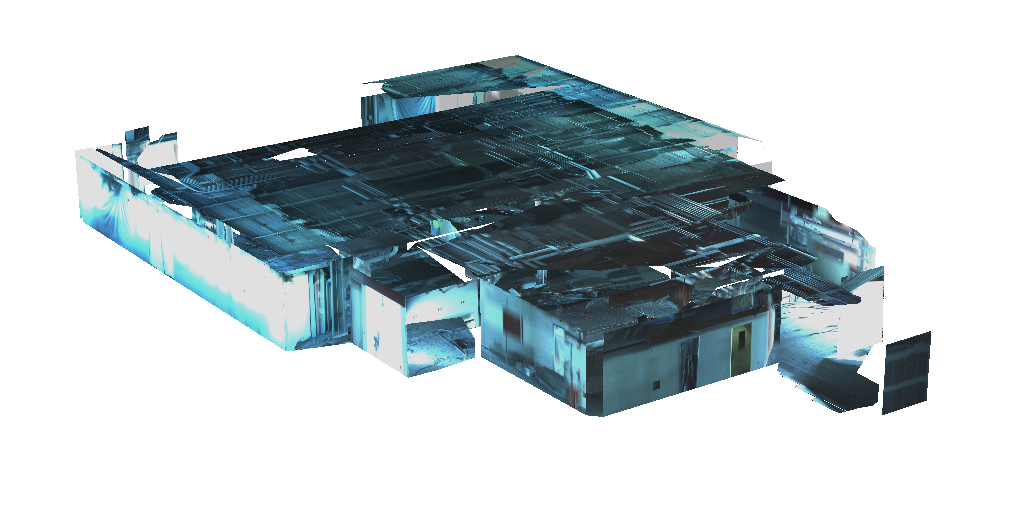
\includegraphics[width=3in]{pier15.png}
  }
  \caption{Textured models from the PCA-based approach.}
  \label{fig:pcaModels}
\end{figure}

\begin{figure}
  \centering{
    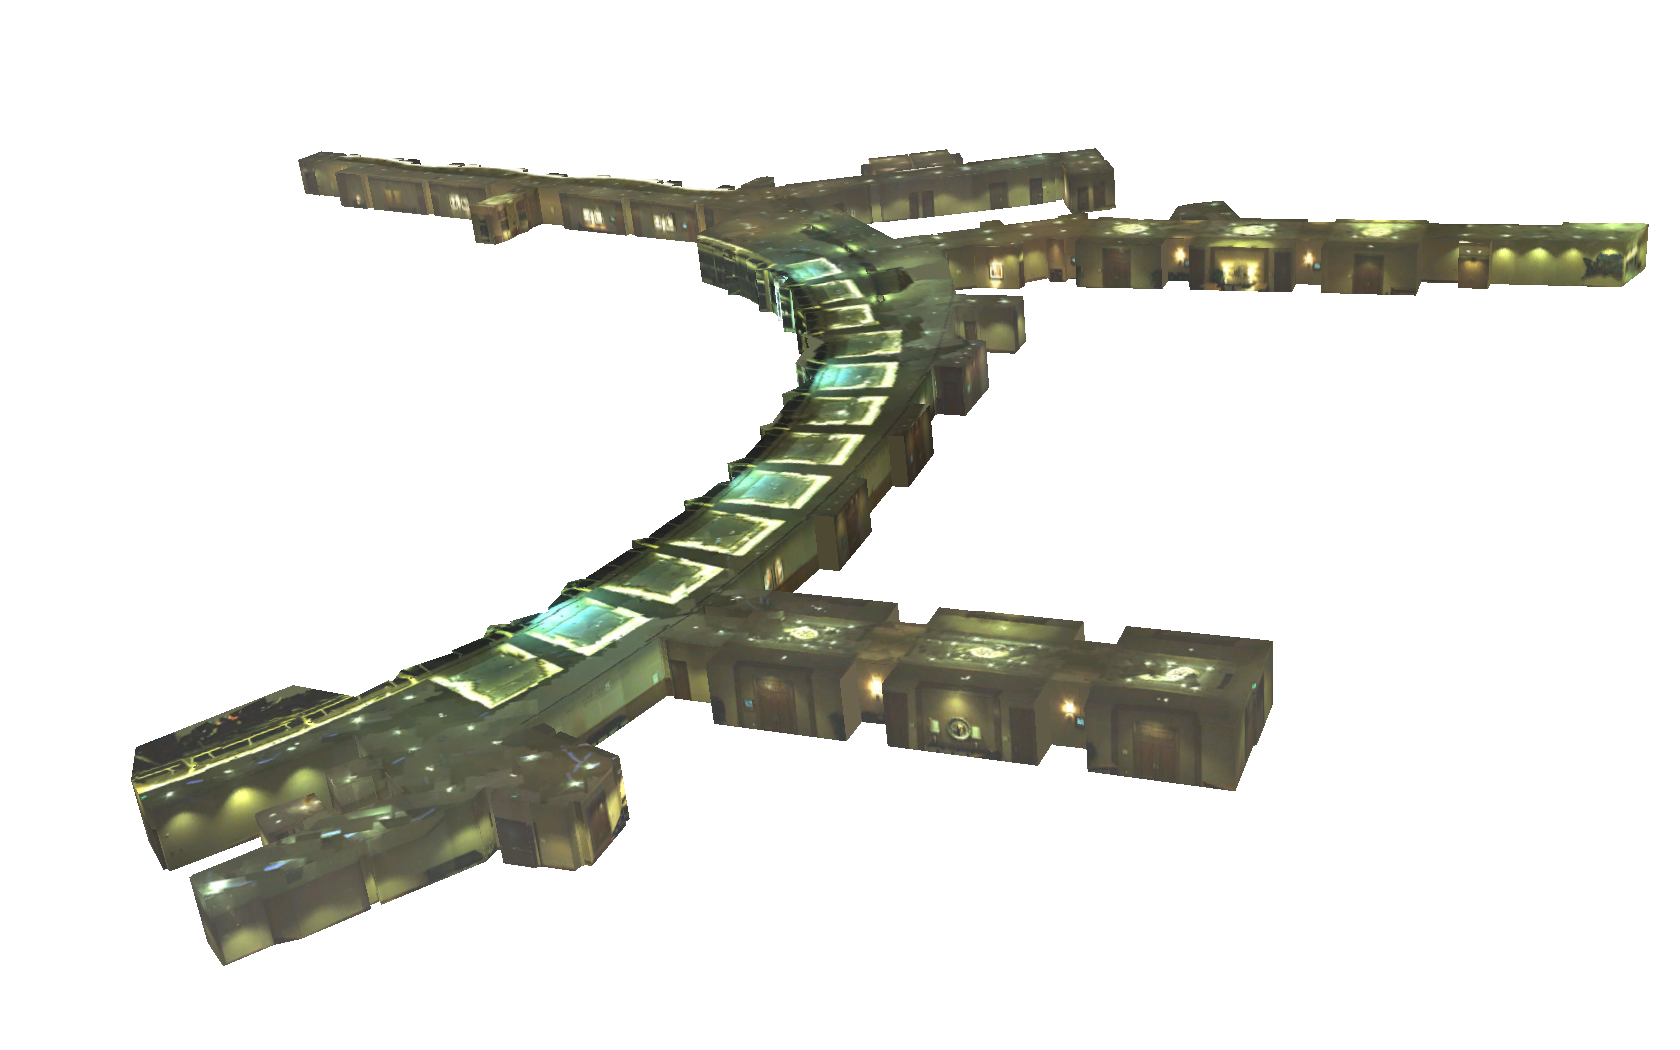
\includegraphics[width=3in]{houston2d1.png}
    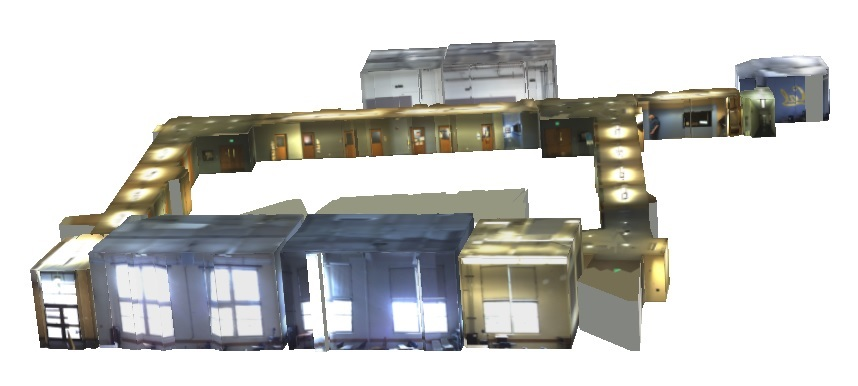
\includegraphics[width=3in]{coryf2.jpg} \\
    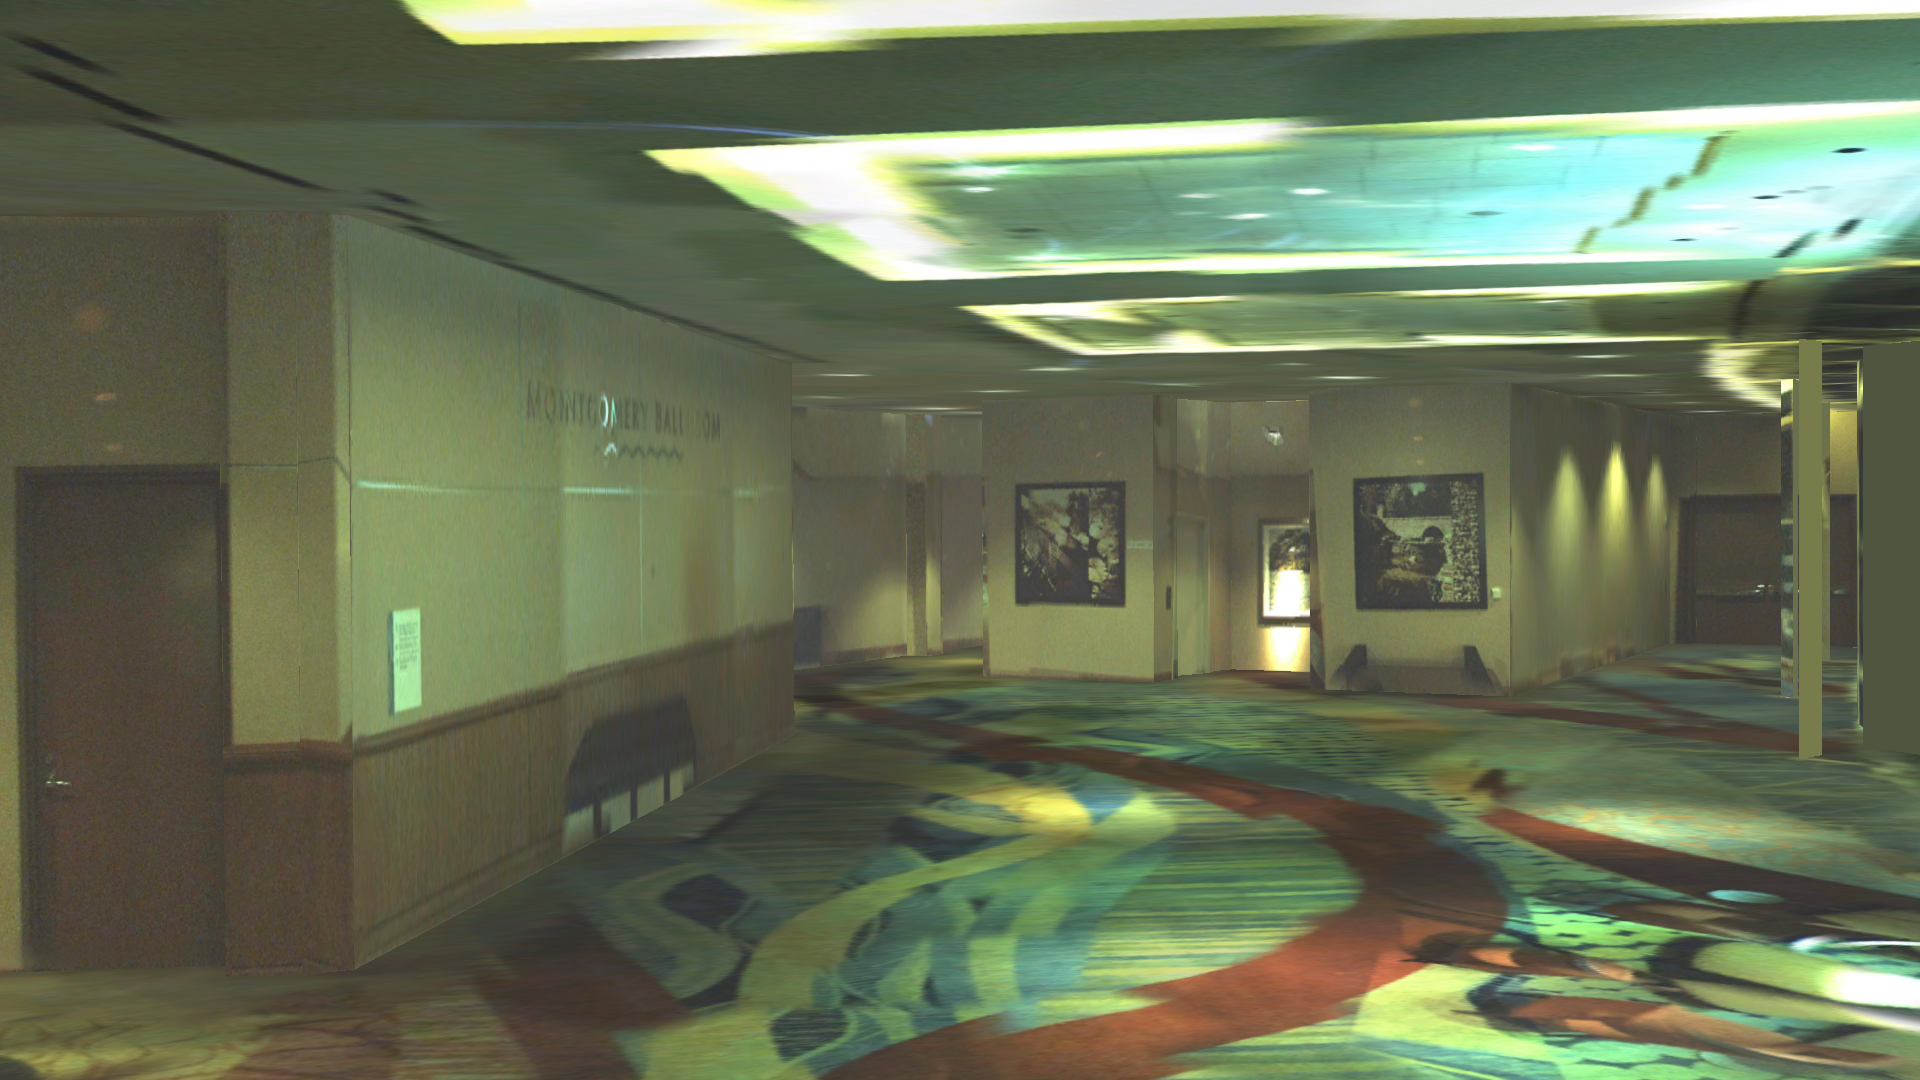
\includegraphics[width=3in]{houston3_2.png}
    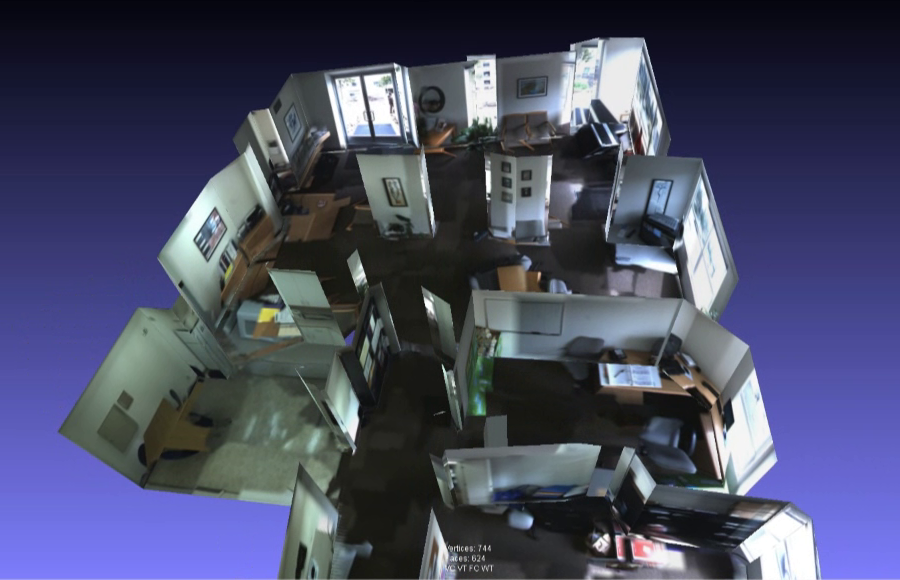
\includegraphics[width=3in]{office.png}
  }
  \caption{Textured models from the floor plan extrusion approach.}
  \label{fig:fpModels}
\end{figure}

\begin{figure}
  \centering{
    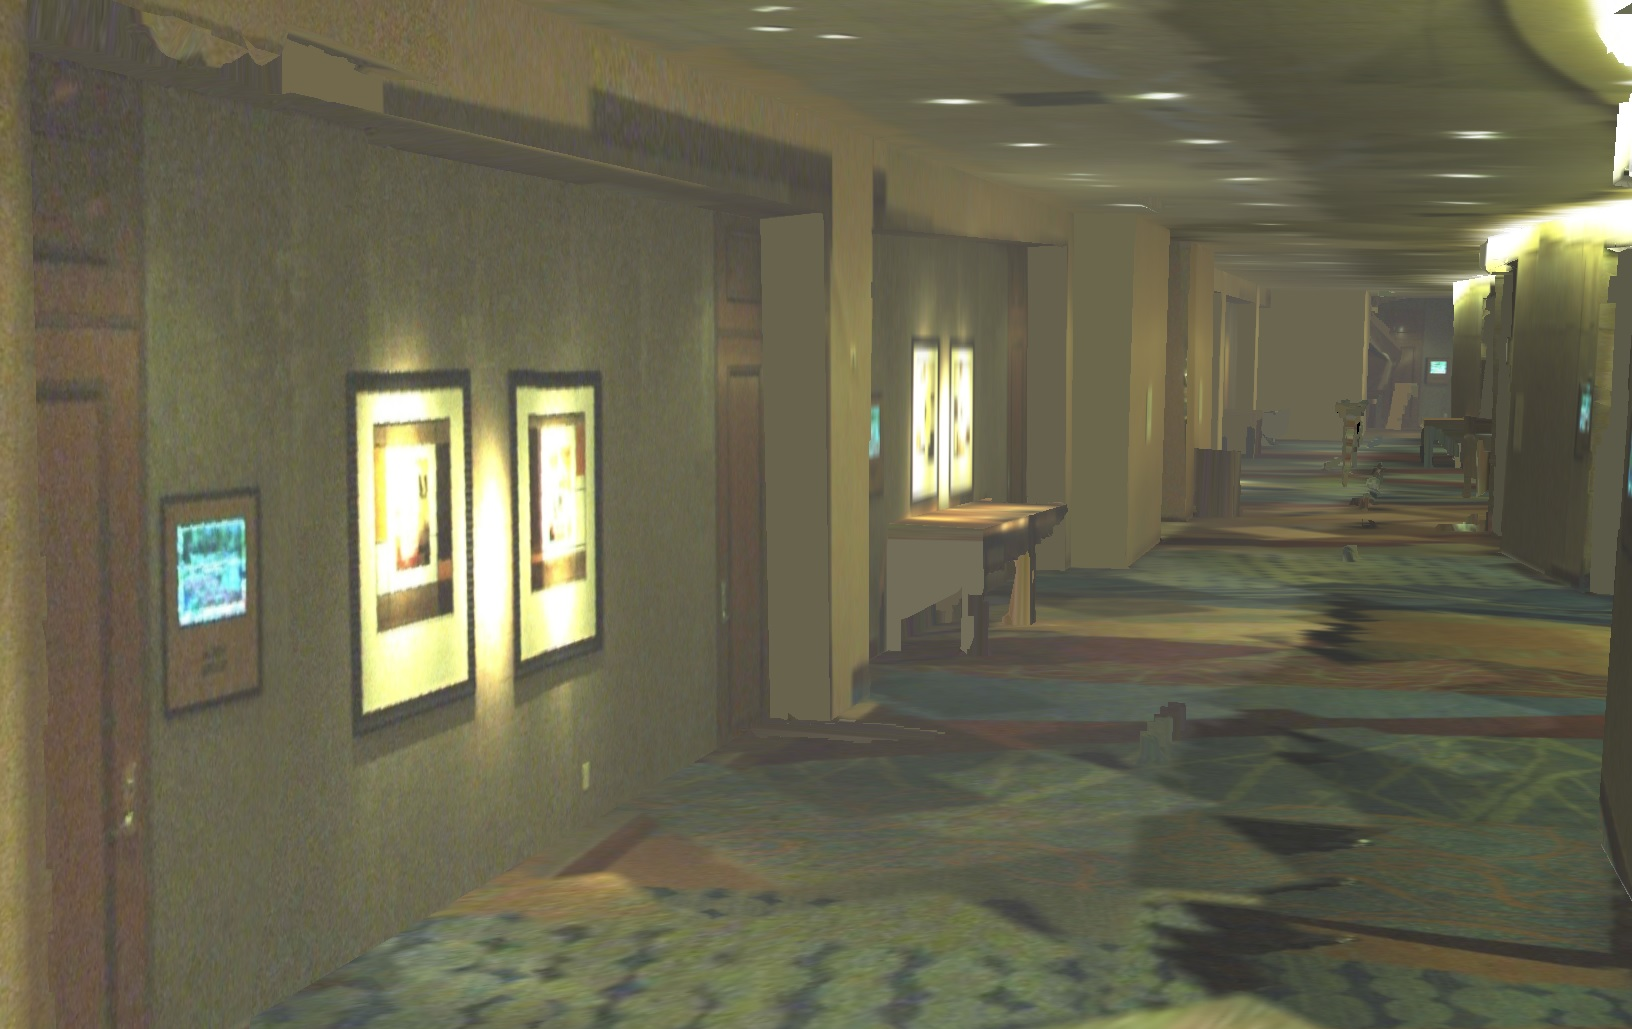
\includegraphics[width=3in]{houston2.jpg}
    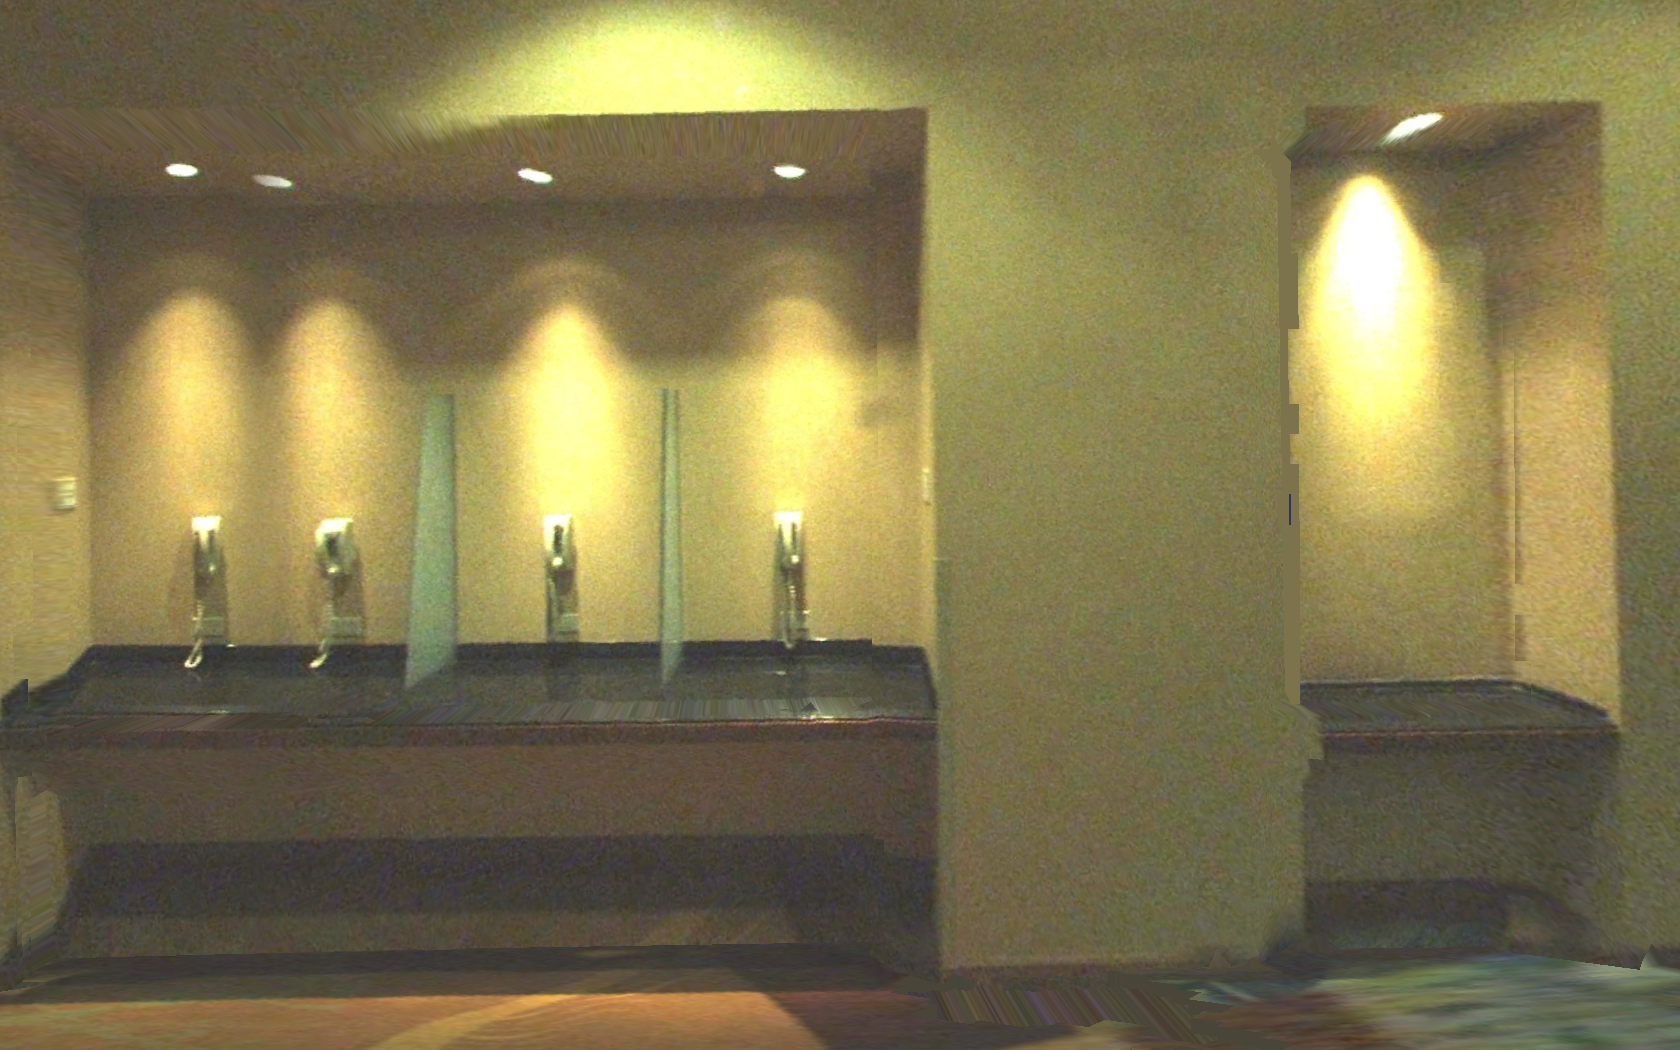
\includegraphics[width=3in]{results_houston_1_3d.png} \\
    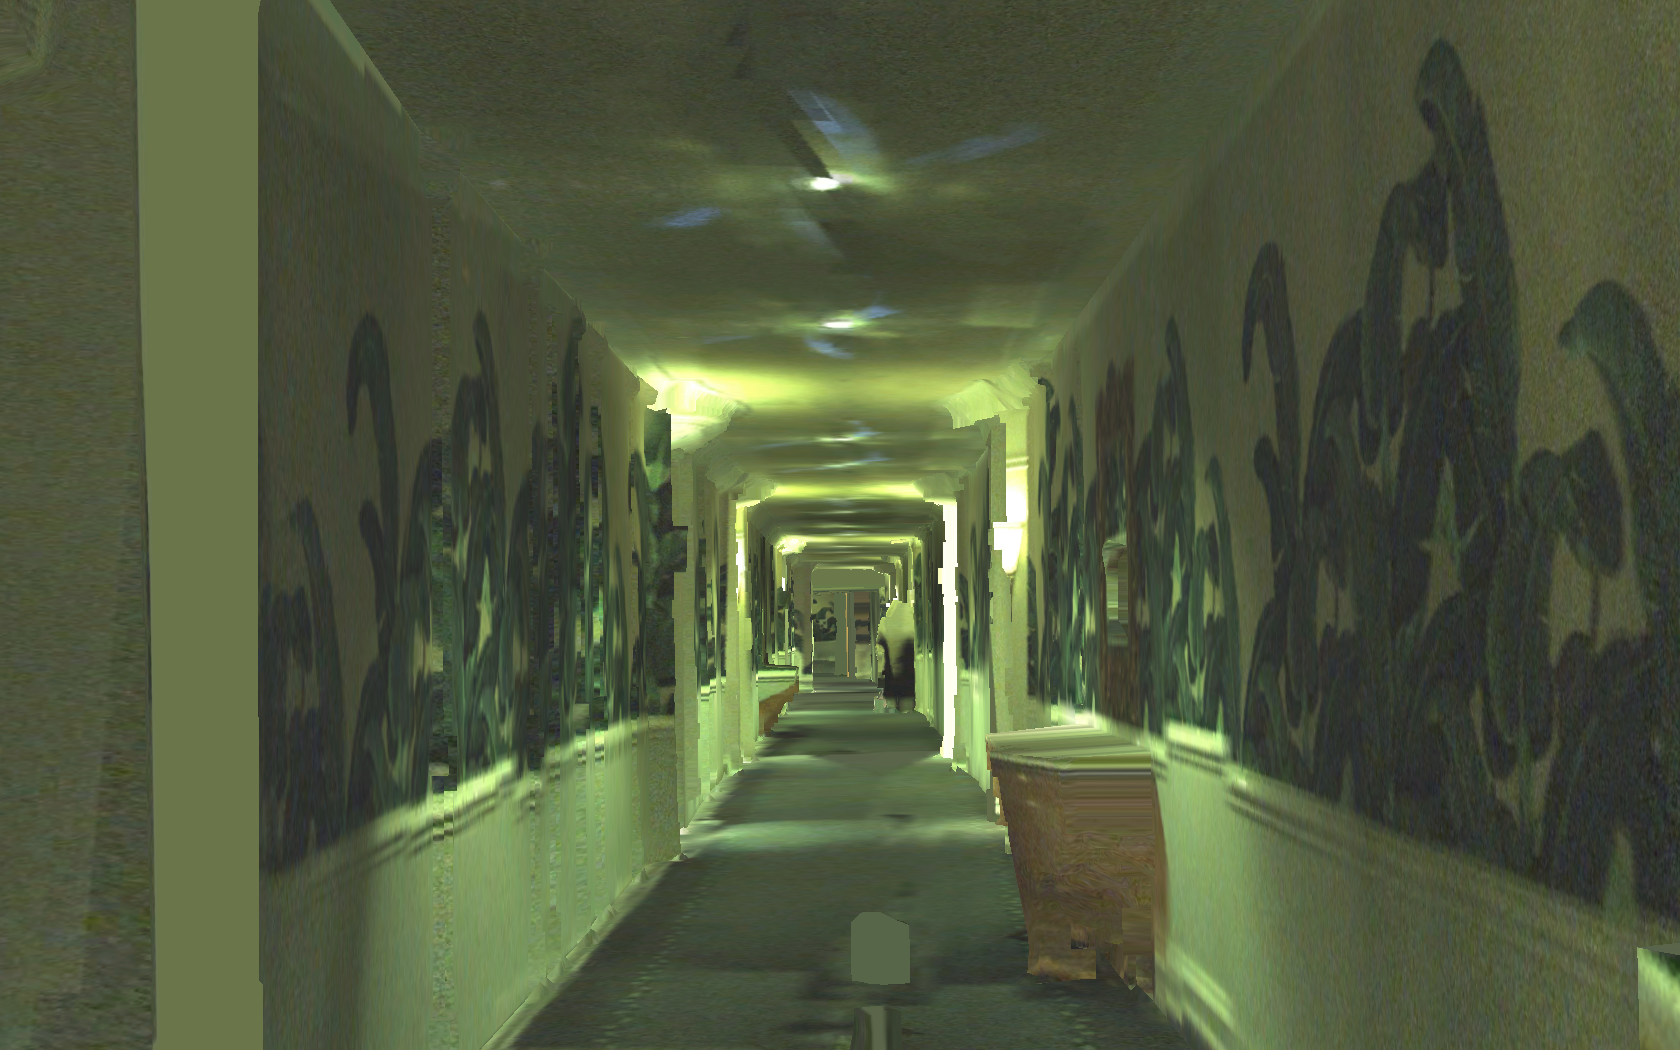
\includegraphics[width=3in]{bhh3d2.png}
    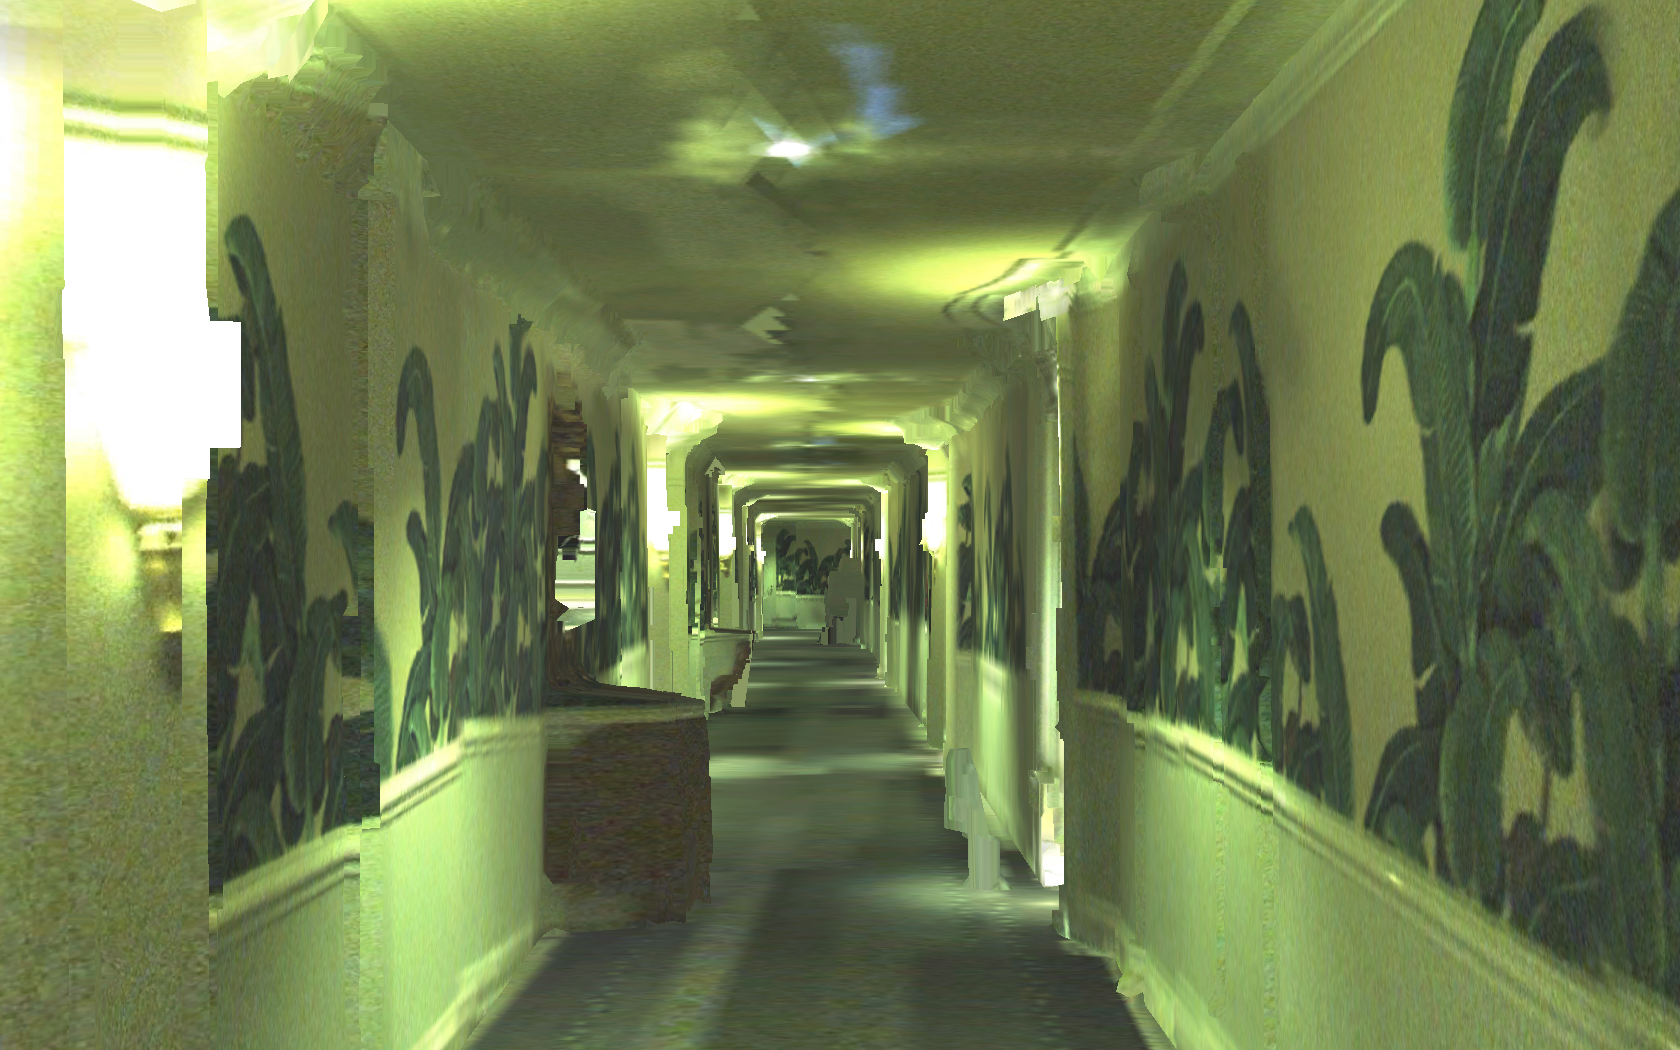
\includegraphics[width=3in]{bhh3d3.png}
  }
  \caption{Textured models from the voxel-carving approach.}
  \label{fig:voxelModels}
\end{figure}



The texture mapping procedure in this paper was tested with three
different geometry-reconstruction methods, a PCA-based plane-fitting
method \cite{sanchez2012point}, a floor plan extrusion method
\cite{turnerfloorplan}, and a voxel-carving mesh generation method
\cite{turnerwatertight}. The first two methods generate very similar
low-resolution models, containing only major walls, ceilings and
floors. The third method generates high-resolution models, and
attempts to reconstruct all scanned objects in the
environment. Texture mapped models generated by the PCA-based, floor
plan extrusion, and voxel-carving approaches, can be seen in Figures
\ref{fig:pcaModels}, \ref{fig:fpModels}, and \ref{fig:voxelModels}
respectively.

\subsection{Runtime}
As mentioned earlier, our approach is quite efficient. The top wall in
Figure \ref{fig:indivPlanes}(a) was generated with 7543 $\times$ 776
pixels, and spans a 40-meter long wall. Given 41000 input images in
the entire dataset, a 2.8 GHz dual-core consumer-grade laptop takes
under a second to choose 36 candidate images, followed by a minute to
perform image projections, image alignment, and the shortest path
texturing method. The tile-caching approach takes roughly comparable
time, and over 75\% of the time for either method is spent on
calculating image projections, which are cached over multiple runs,
and also could be performed as a preprocessing step instead. While not
real-time, the process is capable of generating fast updates after
changes in various parameters or modifications to input data, and if
integrated directly into a 3D modeling system, could provide quick
visual feedback as data is collected.


\subsection{Visualization}
Our full models consist of an input model file, generated textures,
and a mapping of image points to 3D model vertices. The textured
models shown throughout this paper range from 20 MB in size to over
400 MB in a compressed format, with textures of sizes over 500
megapixels. These models are visualized using the OpenSceneGraph
toolkit \cite{openscenegraph}, which allows for export to many common
model formats, as well as interactive visualization, even in web
browsers or mobile devices.

\section{Conclusion}
\label{sec:conclusion}

In this paper, we have developed an approach to texture mapping models
of indoor environments with noisy camera localization data. We are
able to refine image locations based on geometry references and
feature matching, and robustly handle outliers. Using the tile-based
mapping approach, we can texture both large planar features as well as
smaller, more complex surfaces. We also implemented a shortest path
texturing method that produces seamless textures on planes where
multiple head-on images are available. Both of these approaches are
highly modular, and easily tunable for similar systems across multiple
environments.

Our method is likely to fail however in scenarios where 3D error is
large. A logical progression of our approach to resolve camera error
in 3D is to perform matching between image lines and geometry in 3D,
which can be done reasonably efficiently \cite{linebased,
  rectangularstructures}. Using linear features in addition to SIFT
features is also likely to result in improved matches, as indoor
scenes often have long, unbroken lines spanning multiple images
\cite{linearposeestimation}. Finally, the blending procedure is quite
basic, and applying more sophisticated methods of blending as well as
image boundary selection would benefit the final visual quality, and
more robustly handle motion-based or parallax errors.

%%%%%%%%%%%%%%%%%%%%%%%%%%%%%%%%%%%%%%%%%%%%%%%%%%%%%%%%%%%%%
%%%%% References %%%%%

\bibliography{report} %>>>> bibliography data in report.bib
\bibliographystyle{spiebib} %>>>> makes bibtex use spiebib.bst

\end{document} 
